\graphicspath{{./figures}}

\section{Автономные системы}
\subsection{Основные понятия}
Пусть $\Omega \subset \mathbb R^n$ открыто, а функция $f\colon \Omega \to \mathbb R^n$ непрерывно дифференцируема.
Рассмотрим систему
\begin{equation}
    x' = f(x).
\end{equation}

\textbf{Определение.} Такая система называется \textit{автономной}, а $\Omega$ --- это её \textit{фазовое пространство}.

Основная идея такой системы в том, что в правой части нет зависимости от $t$.

\textbf{Определение.} Пусть $x\colon I \to \mathbb R^n$ --- непродолжаемое решение системы (1).
Множество $\{x(t): t \in I\}$ называется \textit{фазовой траекторией}.

\textbf{Определение.} Пусть есть $\widehat x \in \Omega$ такой, что $x(t) \equiv \widehat x$ является решением (1) $\Leftrightarrow f(\widehat x) = 0$.
Тогда вектор $\widehat x$ называется \textit{положением равновесия}.

Рассмотрим несколько примеров.
\begin{enumerate}
    \item Пусть $f\colon \mathbb{R} \to \mathbb{R}$, а также существует единственная точка $\widehat x \in \mathbb{R}:f(\widehat x) = 0$.
    Тогда решение $\widehat{x}$ даёт нам одну фазовую траекторию --- это будет просто одна точка в фазовом пространстве. Кроме того, будут ещё два решения:
    одно будет лежать выше $\widehat{x}$, а другое --- ниже. Можно показать, что их фазовых траектории: это два открытых луча, расходящихся из положения равновесия
    в разные стороны.
    \begin{figure}[h]
        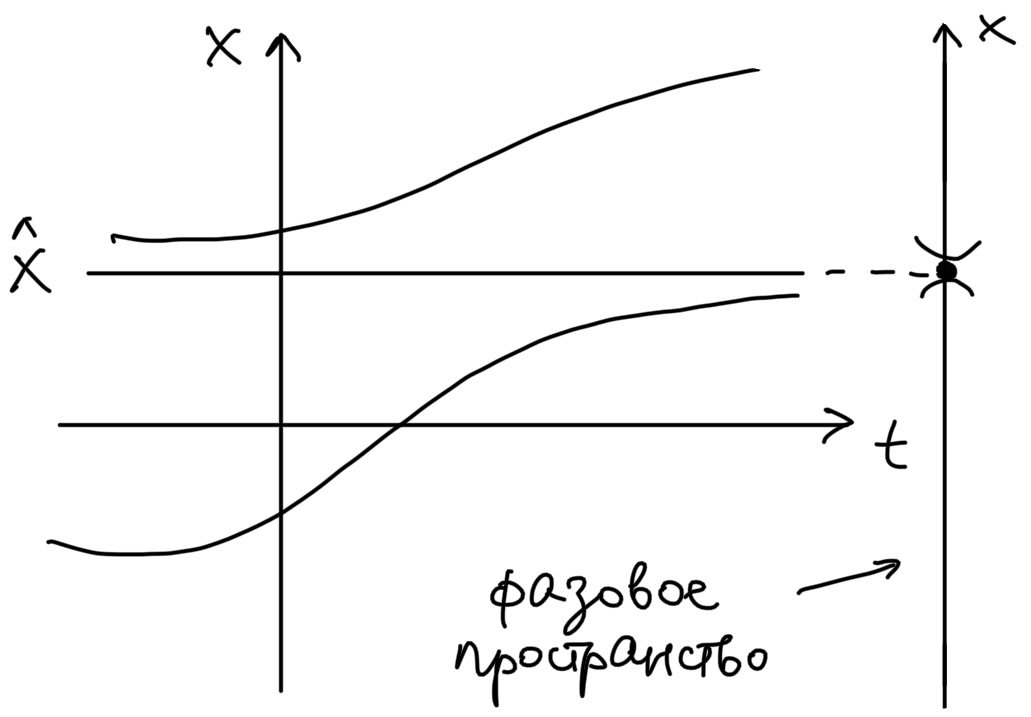
\includegraphics[scale=0.25]{trajectory-example}
        \centering
        \caption{Фазовые траектории}
    \end{figure}
    \item Рассмотрим теперь двумерный случай: $x_1'=x_2$ и $x_2'=-x_1$. Это линейная система, её общее решение: $x_1 = r\cos(t + \alpha)$, $x_2 = r\sin(t + \alpha)$, где $r \geq 0, \alpha \in [0, 2\pi)$.
    В этом случае фазовыми траекториями будут начало координат (положение равновесия) и всевозможные концентрические окружности с центром в начале координат.
\end{enumerate}

\subsection{Свойства автономных систем}
\begin{enumerate}
    \item Еcли $x\colon (a, b) \to \mathbb R^n$ является непродолжаемым решением системы (1), то для любого $c \in \mathbb R$ функция $y(t) \coloneq x(t + c)$, где $t \in (a-c, b-c)$ тоже является непродолжаемым решением.
    
    \textbf{Доказательство.} Для начала покажем, что $y(t)$ является решением (1). Действительно, для $t \in t \in (a-c, b-c)$ имеем:
    $$y'(t) \equiv \frac{d}{dt}x(t+c) \equiv f(x(t+c)) \equiv f(y(t)).$$
    Теперь докажем, что оно непродолжаемое. Предположим противное: пусть $z\colon (d, e) \to \mathbb{R}^n$ является решением (1), причём $(a-c, b-c) \subsetneq (d, e)$, при этом $z(t) \equiv y(t)$ для $t \in (a-c, b-c)$. Тогда функция $z(t-c)$, где $t \in (d + c, e+c)$,
    является решением (1), $(a, b) \subsetneq (d+c, e+c)$, а также $z(t-c) \equiv y(t-c) \equiv x(t) \Rightarrow x$ не является непродолжаемым решением, противоречие.

    \QED

    \item Любые две фазовые траектории $X, Y \in \Omega$ либо не пересекаются, либо совпадают.

        \textbf{Доказательство.} Пусть $X \cap Y \neq \emptyset$. Пусть $x_0 \in X \cap Y$. Переведём на язык решений: для $X$ и $Y$ соответственно существуют непродолжаемые решения $x\colon (a, b) \to \mathbb{R}^n, y\colon (c, d) \to \mathbb{R}^n$, а также точки $t_1 \in (a, b)$ и $t_2 \in (c, d): x(t_1)=x_0=y(t_2)$.
        Возьмём функцию $z(t) \coloneq y(t + t_2 - t_1)$, $t \in (c - t_2 + t_1, d - t_2 + t_1)$, тогда по первому свойству она является непродолжаемым решением (1). При $t=t_1$ получаем $y(t + t_2 - t_1) = x_0$. Значит, $z(t)$ является решением задачи Коши
        \begin{equation}
            \begin{cases}
                x' = f(x) \\
                x(t_1) = x_0
            \end{cases}.
            \nonumber
        \end{equation}
        Заметим, что $x$ тоже является непродолжаемым решением этой задачи, а тогда по теореме о существовании и единственности $$x(t) \equiv z(t) \Rightarrow X = \{z(t) : t \in (c-t_2+t_1, d-t_2+t_1)\} = Y.$$

        \QED

        \textbf{Следствие.} Решение автономной системы не достигает положения равновесия за конечное время.
        
        Понимать это можно следующим образом. Вспомним картинку из примера 1. Возьмём один из получившихся лучей в фазовом пространстве. Ему соответствует какое-то решение $x(t)$. Начнём подставлять в $x(t)$ разные $t$. Если для какого-то $t_0$ мы попадём в положение равновесия, то
        у нас пересекутся две фазовые траектории: выбранный луч и сама точка положения равновесия. Тогда они должны совпадать, но это невозможно. Поэтому ни для какого конечного $t$ мы не попадём в положение равновесия.

    \item Пусть $x\colon \mathbb R \to \mathbb R^n$ ---  непродолжаемое решение (1).
        Предположим, что нашлись $t_1 < t_2: x(t_1) = x(t_2)$, причём $x(t) \not\equiv$ const.
        Тогда функция $x$ --- это периодическая функция с положительным наименьшим периодом, а её фазовая траектория является замкнутой кривой без самопересечений.

        \textbf{Доказательство.} Возьмём функцию $y(t) \coloneq x(t + t_2 - t_1), t\in \mathbb{R}$, она является непродолжаемым решением (1).
        Более того, $y(t_1) = x(t_2) = x(t_1)$, а тогда функции $x$ и $y$ являются решениями одной и той же задачи Коши $\Rightarrow$ по теореме о существовании и единственности $y(t) \equiv x(t)$.
        Положим $d = t_2 - t_1$, тогда это тождество переписывается в виде $x(t) \equiv x(t + d)$.
        Пусть $P$ --- это множество всех периодов функции $x$. Мы знаем, что оно непусто, так как $d \in P$.

        Так как $x(t) \not\equiv$ const, то существует $\tau \in \mathbb{R}: x(\tau) \neq x(t_1)$. Пусть $\varepsilon = \frac{1}{2}|x(\tau) - x(t_1)|$. В силу непрерывности функции $x$ существует $\delta > 0: x(t) \in (x(\tau) - \varepsilon, x(\tau) + \varepsilon)$ для любого $t \in (\tau - \delta, \tau + \delta)$.
        В силу выбора $\varepsilon$ получаем, что $x(t) \neq x(t_1)$ для любого $t \in (\tau - \delta, \tau + \delta) \Rightarrow$ для любого $p \in P$ имеем $p > \delta$, а тогда $\widehat{p} \coloneq \inf P \geq \delta > 0$.
        Докажем теперь, что $\widehat p \in P$.
        Для этого рассмотрим последовательность $\{p_j\} \subset P$ такую, что $p_j \to \widehat p$ при $j \to \infty$.
        Тогда для любого $j$ имеем $x(t + p_j) \equiv x(t)$.
        Переходя к пределу по $j$ и пользуясь непрерывностью функции $x$, получаем, что $x(t + \widehat p) \equiv x(t)$, то есть $\widehat p \in P$. Таким образом, мы показали, что существует положительный наименьший период.

        Осталось доказать, что фазовая траектория $X$ функции $x$ не имеет самопересечений, то есть для любых $\widehat t_1, \widehat t_2 \in \mathbb{R} : |\widehat t_1 - \widehat t_2| < \widehat{p}$ выполняется $x(\widehat t_1) \neq x(\widehat t_2)$.
        Предположим противное: пусть существуют $\widehat t_1, \widehat t_2 \in \mathbb{R}: \widehat t_1 < \widehat t_2, \widehat t_2 - \widehat t_1 < \widehat p$, при этом $x(\widehat t_1) = x(\widehat t_2)$. Тогда из начала доказательства получаем, что $\widehat t_2 - \widehat t_1 \in P$. Но тогда получаем противоречие с минимальностью $\widehat p$.

        \QED

    \item Вывод: траектория --- это либо точка, либо замкнутая кривая без самопересечений, либо незамкнутая кривая без самопересечений.


    \item (групповое свойство автономной системы) Рассмотрим задачу Коши
        \begin{equation}
            \begin{cases}
                x' = f(x) \\
                x(0) = x_0
            \end{cases}.
        \end{equation}
        Обозначим через $\phi(t, x_0)$ непродолжаемое решение (2), $x_0 \in \Omega$, $t \in \mathbb{R}$.
    Тогда справедливо тождество $\phi(t, \phi(\tau, x_0)) \equiv \phi(t + \tau, x_0)$.
        
        % \begin{figure}[ht]
        %     \centering
        %     \incfig{4-1}{0.75\linewidth}
        %     \caption{Групповое свойство}
        % \end{figure}

        % Как это представлять: вот у нас есть какая-то траектория, стартующая из точки $\xi$.
        % В точке $s$ она находится в какой-то точке $\phi(s, \xi)$, и из этой точки, как из стартовой, можно пустить ещё одну траекторию, которая в точке $t$ примет значение $\phi(t, \phi(s, \xi))$.
        % Но то же самое значение примет и исходная траектория в точке $s + t$.

        % И при чём тут группы: рассмотрим отображения $\phi(t, \cdot): \mathbb R^n \to \mathbb R^n$ (здесь $t$ --- параметр).
        % Зададим операцию $\phi(t, \cdot) \circ \phi(s, \cdot) = \phi(t, \phi(s, \cdot))$.
        % И вот по групповому свойству множество таких отображений является абелевой группой с единицей $\phi(0, \cdot)$.

        \textbf{Доказательство.} Зафиксируем $\tau$. Тогда по свойству 1 функция $\phi(t + \tau, x_0)$ является решением системы (1).
        В то же время по определению $\phi(t, \phi(\tau, \xi))$ тоже является решением (1).
        Рассмотрим $t = 0$: тогда в левой части имеем $\phi(0, \phi(\tau, x_0)) = \phi(\tau, x_0)$, в правой --- $\phi(0 + \tau, x_0) = \phi(\tau, x_0)$.
        То есть в $t=0$ решения совпадают, а тогда по теореме о существовании и единственности для любого $\tau$ выполняется $\phi(t + \tau, x_0) \equiv \phi(t, \phi(\tau, x_0))$.

        \QED

    \item Функция $\phi$ непрерывна.
    
    Это верно в силу теоремы о непрерывной зависимости непродолжаемого решения задачи Коши от начального условия и параметра, которая доказывалась в прошлом семестре.

    \item Рассмотрим множество отображений $\Phi \coloneq \{\phi(t, \cdot) \colon \Omega \to \Omega \;|\; t \in \mathbb{R}\}$. Зададим операцию композиции: $\phi(t, \cdot) \circ \phi(s, \cdot) = \phi(t, \phi(s, \cdot))$. Тогда $(\Phi, \circ)$ --- это абелева группа.

    \textbf{Доказательство.} Здесь нам помогает групповое свойство, которое мы только что доказали. Запишем следующее равенство: $$\phi(t, \phi(s, \cdot)) \equiv \phi(t + s, \cdot) \equiv \phi(s, \phi(t, \cdot)).$$
    Из него получаем, что $\Phi$ замкнуто относительно композиции и операция коммутативна. Это же равенство показывает, что нейтральным элементом будет $\phi(0, \cdot)$, а обратным к $\phi(t, \cdot)$ будет $\phi(-t, \cdot)$.

    \QED

\end{enumerate}

% \subsection{Предельные множества траекторий}
% Пусть $x: (t_0, +\infty) \to \mathbb R^n$ --- решение системы (1), $T$ --- его траектория.

% \textbf{Определение.} $a \in \mathbb R^n$ называется \textit{$\omega$-предельной точкой} (траектории $T$), если существует последовательность $\{t_j\} \to +\infty$, такая что $x(t_j) \to a$ при $j \to +\infty$.

% Обозначим через $\Omega(T)$ \textit{$\omega$-предельное множество} --- множество всех $\omega$-предельных точек траектории $T$.

% \textbf{Пример 1.} Пусть $n = 1$, $t_0 = 0$ и $x' = x$.
% Рассмотрим решение $x(t) = e^t$, тогда $T = (1, +\infty)$.
% Тогда $\Omega(T) = \varnothing$.

% \textbf{Пример 2.} То же самое, но $x' = -x$ и $x = e^{-t}$.
% Тогда $T = (0, 1)$ и $\Omega(T) = \{0\}$.

% \textbf{Теорема.} (б/д) Пусть $T$ ограничена и найдётся $\varepsilon > 0$, такое что $\varepsilon$-окрестность траектории $T$ вложена в $\Sigma$ (то есть вложено с запасом).
% Тогда $\Omega(T)$ непусто, ограничено, замкнуто, связно и состоит из траекторий, то есть является дизъюнктным объединением каких-то траекторий.

% \textbf{Теорема.} (Бендиксона, б/д) Предположим, что $n = 2$, $\Omega(T)$ ограничено и непусто, и на нём $f(x) \ne 0$, то есть не содержит положения равновесия.
% Тогда $\Omega(T)$ --- это замкнутая траектория.

\setcounter{equation}{0}
\section{Автономные системы на плоскости}
\subsection{Линейные автономные системы}
Нам дана невырожденная матрица $A \in \mathbb{R}^{2 \times 2}$. Рассмотрим автономную систему $x' = Ax$:
\begin{equation}
    \begin{cases}
        x_1' = a_{11} x_1 + a_{12} x_2 \\
        x_2' = a_{21} x_1 + a_{22} x_2
    \end{cases}.
\end{equation}
У неё гарантированно есть положение равновесия $x = 0$. Чтобы понять, как система ведёт себя в окрестности нулевого положения равновесия, посмотрим на собственные значения $\lambda_1, \lambda_2$ матрицы $A$.

\textbf{Примечание.} Для удобства все фазовые портреты будем строить в системе координат для базиса $(h_1, h_2)$. Направление движения можно определить, устремив $t \to +\infty$. Кроме того, помним, что фазовые траектории не пересекаются.

\subsubsection{$\lambda_1, \lambda_2 \in \mathbb R \setminus \{0\}$, $\lambda_1 \ne \lambda_2$}
Пусть $h_1$ и $h_2$ --- соответствующие собственные векторы.
Тогда в базисе $(h_1, h_2)$ система будет иметь вид
\[
    \begin{cases}
        y_1' = \lambda_1 y_1 \\
        y_2' = \lambda_2 y_2
    \end{cases}
\]
и её решением будет
\[
    \begin{cases}
        y_1 = c_1 e^{\lambda_1 t} \\
        y_2 = c_2 e^{\lambda_2 t}
    \end{cases} .
\]
Напишем уравнение её траектории, исключив параметр $t$:
\[
    e^{\lambda_1 t} = \frac{y_1}{c_1} \Rightarrow y_2 = c_2(e^{\lambda_1 t})^{\frac{\lambda_2}{\lambda_1}} = c_2 \left(\frac{y_1}{c_1} \right)^{\frac{\lambda_2}{\lambda_1}}
\]
при $c_1 \ne 0$, а при $c_1 = 0$ получится уравнение $y_1 = 0$.

\begin{itemize}
\item Первый случай: $\lambda_1 \cdot \lambda_2 > 0$.
На рисунке 2 слева изображён портрет для случая $\lambda_2 > \lambda_1 > 0$, а справа для случая $\lambda_1 > \lambda_2 > 0$.

\begin{figure}[h]
    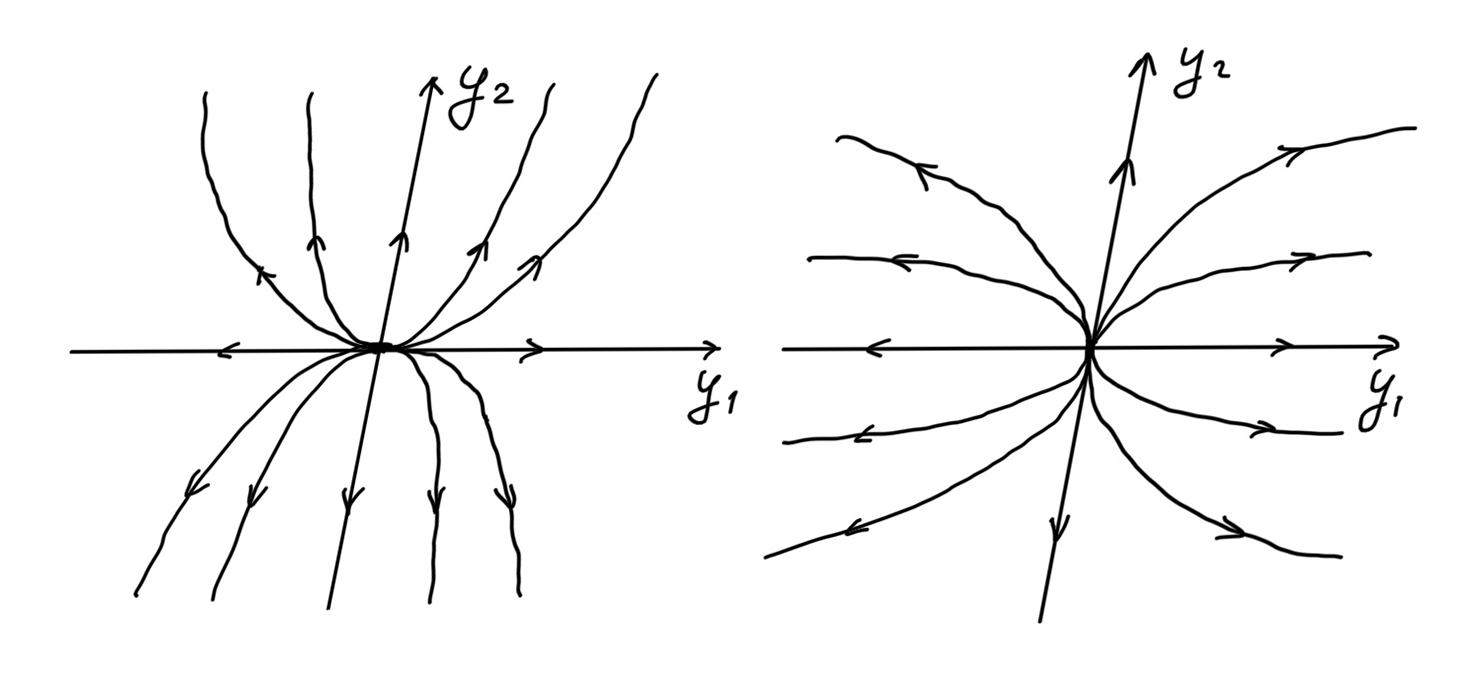
\includegraphics[scale=0.25]{unstable-knot}
    \centering
    \caption{Неустойчивый узел}
\end{figure}

\textbf{Определение.} Полученный портрет называется \textit{неустойчивым узлом}.

Если $\lambda_2 < \lambda_1 < 0$ или $\lambda_1 < \lambda_2 < 0$, то получатся аналогичные портреты, но с направлением к началу координат.

\textbf{Определение.} Тогда портрет называется \textit{устойчивым узлом}.

Устойчивость означает, что при $t \to +\infty$ точка движется к положению равновесия.

\item Второй случай: $\lambda_1 \cdot \lambda_2 < 0$. На рисунке 3 слева изображён портрет для случая $\lambda_1 < 0, \lambda_2 > 0$, а справа для случая $\lambda_1 > 0, \lambda_2 < 0$.

\begin{figure}[h]
    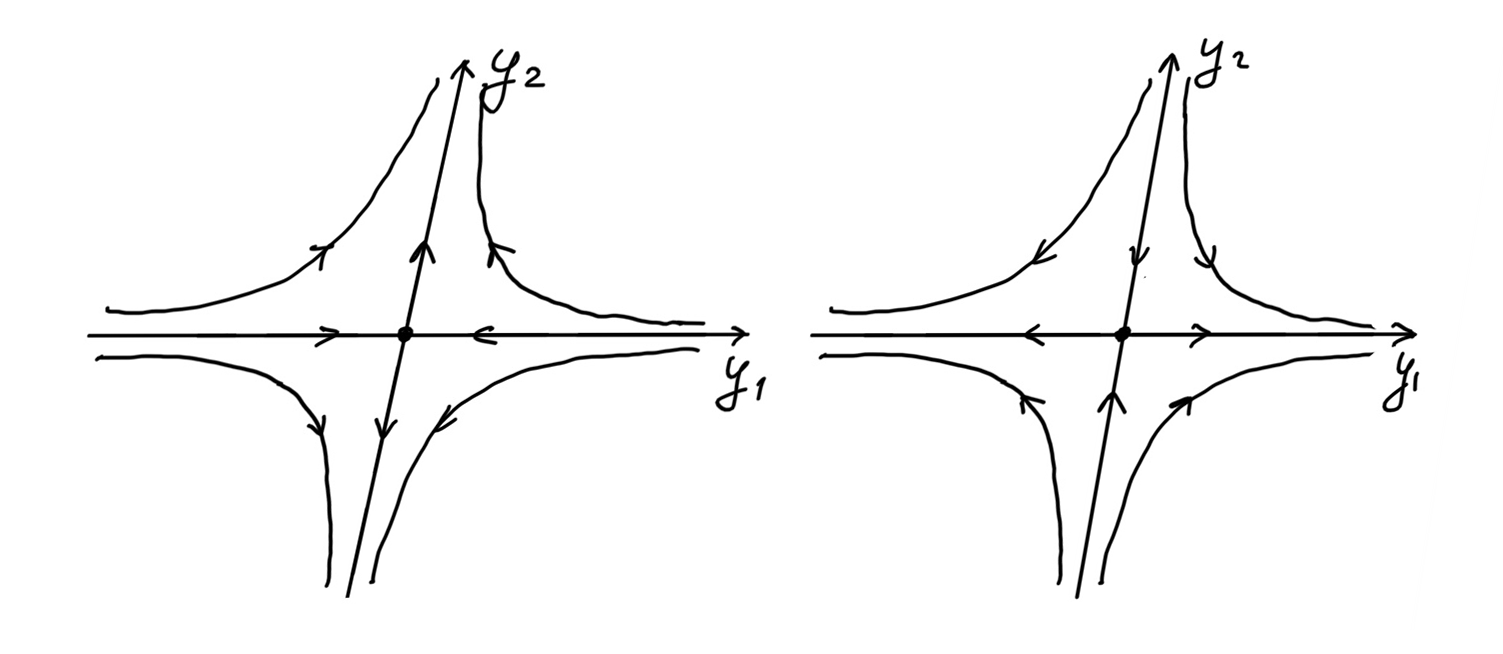
\includegraphics[scale=0.25]{seat}
    \centering
    \caption{Седло}
\end{figure}

\textbf{Определение.} Полученный портрет называется \textit{седлом}.
\end{itemize}

\subsubsection{$\lambda_1 = \lambda_2 = \lambda \in \mathbb R$}
\begin{itemize}
\item Первый случай: $A$ имеет два линейно независимых собственных вектора $h_1$ и $h_2$.
Тогда аналогично прошлым рассуждениям получаем, что кривая имеет вид
\[
    \begin{cases}
        y_2 = \frac{c_2}{c_1} y_1, & c_1 \ne 0 \\
        y_1 = 0, & c_1 = 0
    \end{cases}.
\]
На рисунке 4 слева изображён портрет для случая $\lambda > 0$, а справа для случая $\lambda < 0$.

\begin{figure}[h]
    \includegraphics[scale=0.25]{dicritical-knot}
    \centering
    \caption{Дикритический узел}
\end{figure}

\textbf{Определение.} Полученный портрет называется \textit{дикритическим узлом}.
При $\lambda > 0$ он называется \textit{неустойчивым}, а при $\lambda < 0$ --- \textit{устойчивым}.

\item Второй случай: $h_1$ --- собственный вектор, $h_2$ --- присоединённый к нему.
Тогда в базисе $(h_1, h_2)$ система будет иметь вид
\[
    \begin{cases}
        y_1' = \lambda y_1 + y_2 \\
        y_2' = \lambda y_2
    \end{cases}.
\]
Найдём решение:
\[
    \begin{cases}
        y_1 = c_1 e^{\lambda t} + c_2 t e^{\lambda t} \\
        y_2 = c_1 e^{\lambda t}
    \end{cases}.
\]
Выразим $t$ (считаем, что $c_2 \ne 0$):
\[
    e^{\lambda t} = \frac{y_2}{c_2} \Rightarrow t = \frac{1}{\lambda} \ln \left( \frac{y_2}{c_2} \right).
\]
Подставим в первое уравнение:
\[
    y_1 = c_1 \frac{y_2}{c_2} + \frac{c_2}{\lambda} \ln \left( \frac{y_2}{c_2} \right) \frac{y_2}{c_2}.
\]
На рисунке 5 слева изображён портрет для случая $\lambda > 0$, а справа для случая $\lambda < 0$.
\pagebreak
\begin{figure}[h]
    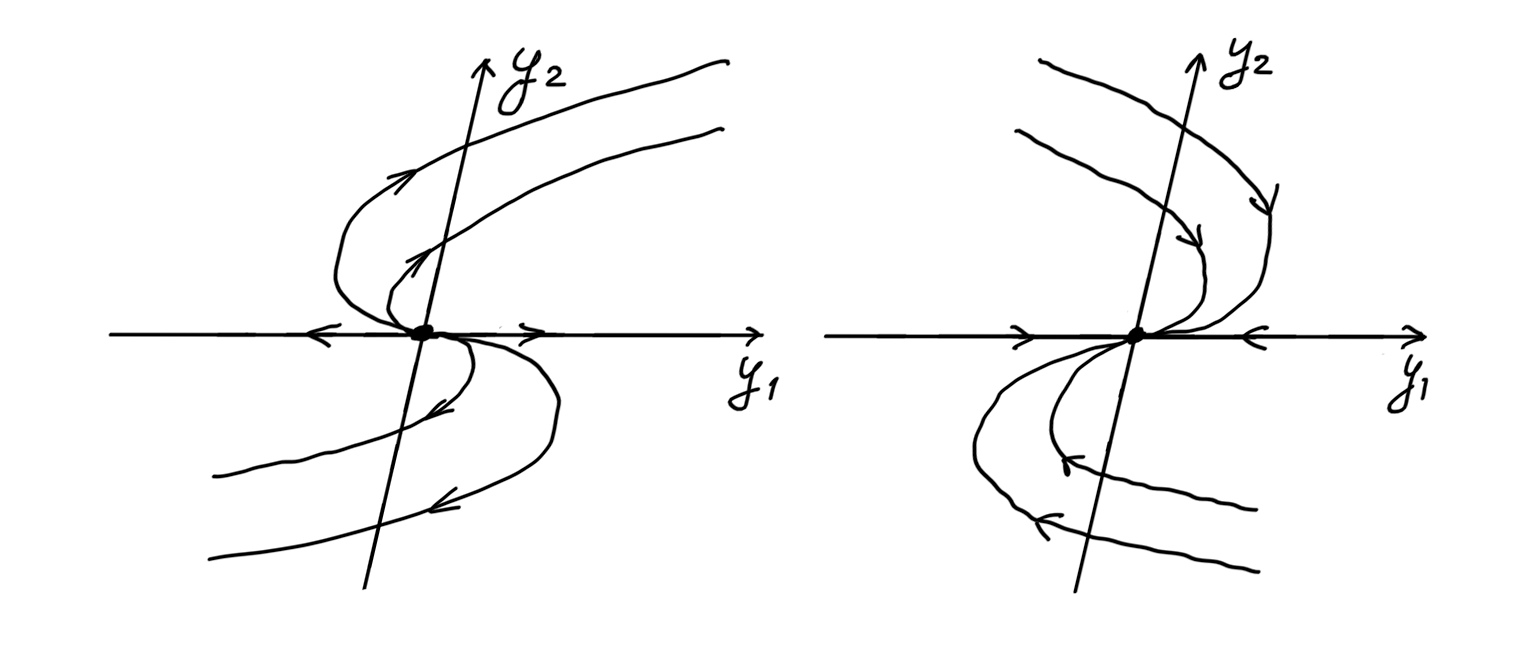
\includegraphics[scale=0.25]{degenerate-knot}
    \centering
    \caption{Вырожденный узел}
\end{figure}
\end{itemize}

\textbf{Определение.} Этот портрет называется \textit{вырожденным узлом}. При $\lambda > 0$ он называется \textit{неустойчивым}, а при $\lambda < 0$ --- \textit{устойчивым}.

\subsubsection{$\lambda_{1, 2} = \alpha \pm \beta i \in \mathbb{C}$, $\beta \neq 0$}
Тогда собственные векторы имеют вид $h_{1,2} = a \pm b i$, где $a$ и $b$ --- линейно независимые векторы.
Как известно, фундаментальной системой решений здесь будет
\[
    \begin{cases}
        v_1 = e^{\alpha t}(a \cos(\beta t) - b \sin(\beta t))\\
        v_2 = e^{\alpha t}(a \sin(\beta t) + b \cos(\beta t))
    \end{cases}
\]
В базисе $(a, b)$ она имеет вид
\[
    \begin{cases}
        y_1 = e^{\alpha t}
        \begin{pmatrix}
            \cos(\beta t) \\
            -\sin(\beta t)
        \end{pmatrix} \\\\

        y_2 = e^{\alpha t}
        \begin{pmatrix}
            \sin(\beta t) \\
            \cos(\beta t)
        \end{pmatrix}
    \end{cases}
\]
Тогда общее решение имеет вид
\[
    y(t) = r e^{\alpha t}
    \begin{pmatrix}
        \cos(\beta (t - \theta)) \\
        \sin(\beta (t - \theta))
    \end{pmatrix}.
\]
для всех $r$ и $\theta$. Чтобы получить его, нужно просто расписать $c_1 y_1 + c_2 y_2$ с помощью формул косинуса суммы, синуса суммы и дополнительного угла.

\begin{itemize}
\item При $\alpha = 0$ получается уравнение окружности. На рисунке 6 слева изображён портрет для случая $\beta > 0$, а справа для случая $\beta < 0$.
\pagebreak

\begin{figure}[h]
    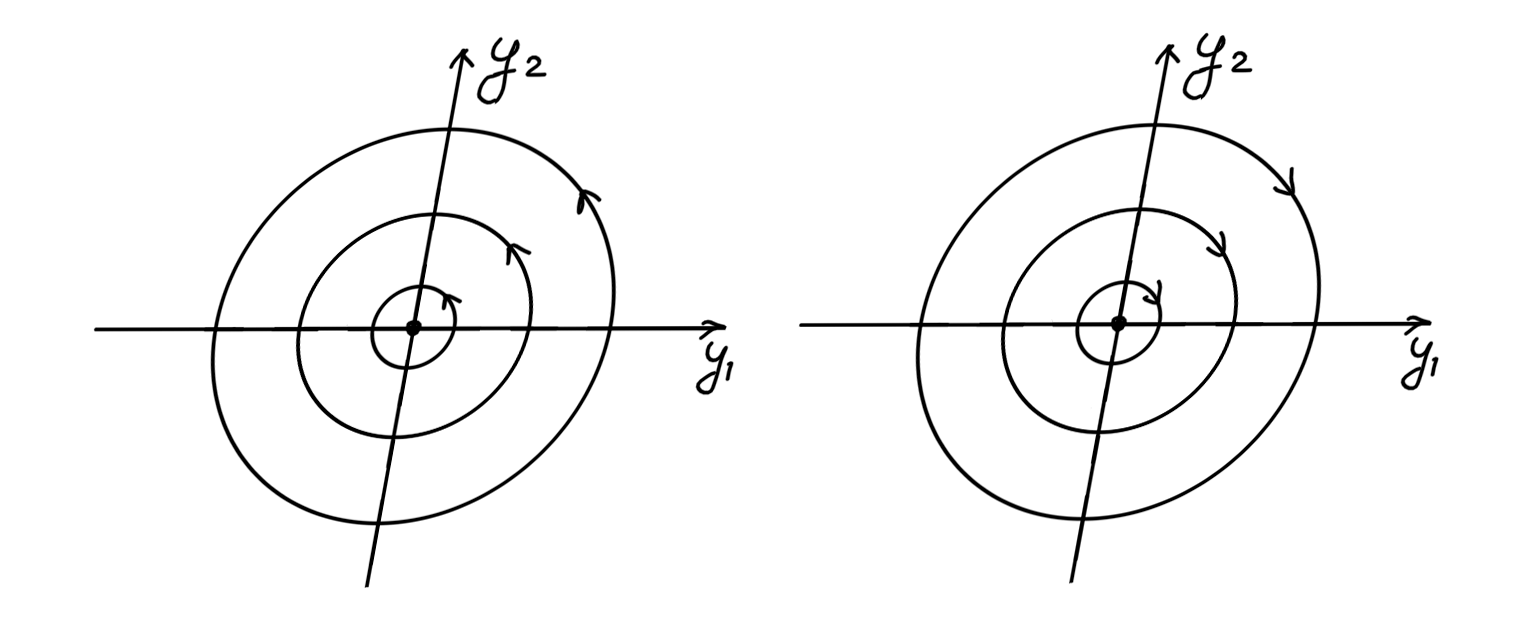
\includegraphics[scale=0.25]{center}
    \centering
    \caption{Центр}
\end{figure}

\textbf{Определение.} Такой портрет называется \textit{центром}.

\item При $\alpha > 0$ расстояние от начала координат увеличивается при $t \to +\infty$, а ещё меняется угол, поэтому получается спираль, как на рисунке 7, вращающаяся против часовой стрелки при $\beta > 0$ (изображена слева) и по часовой при $\beta < 0$ (изображена справа).
В окрестности нуля (при $t \to -\infty$) происходит бесконечное число витков, поэтому там обычно график не рисуют.

\begin{figure}[h]
    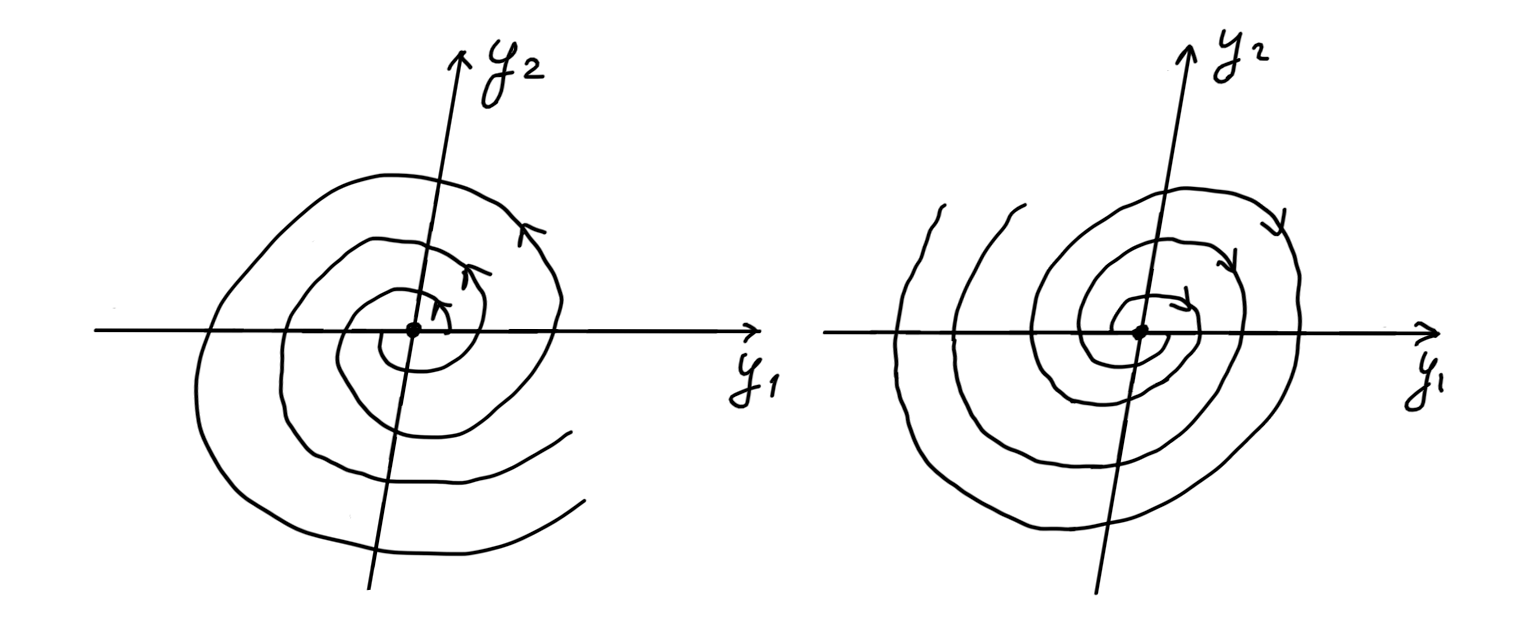
\includegraphics[scale=0.25]{unstable-focus}
    \centering
    \caption{Неустойчивый фокус}
\end{figure}

\textbf{Определение.} Полученный портрет называется \textit{неустойчивым фокусом}.

\item При $\alpha < 0$ получается всё то же самое, но теперь всё наоборот: направление к началу координат, при $\beta > 0$ спираль вращается по часовой стрелке (изображена справа), а при $\beta < 0$ --- против часовой (изображена слева).
\pagebreak
\begin{figure}[h]
    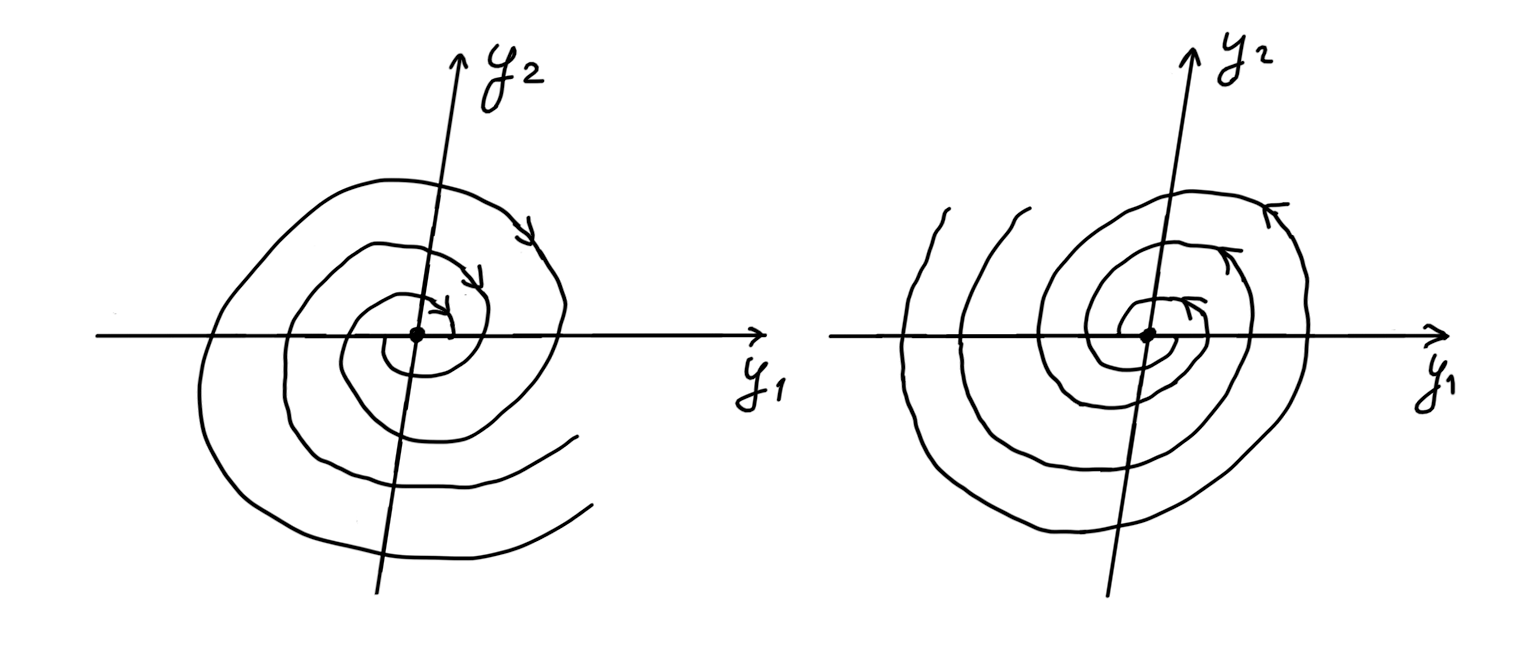
\includegraphics[scale=0.25]{stable-focus}
    \centering
    \caption{Устойчивый фокус}
\end{figure}

\textbf{Определение.} Полученный портрет называется \textit{устойчивым фокусом}.
\end{itemize}

Вообще говоря, есть ещё один случай: когда матрица $A$ вырождена, но он нас интересовать не будет, так как при исследовании нелинейных систем нам будет нужна невырожденность.

\subsection{Нелинейные автономные системы}
Пусть нам даны открытое множество $\Omega \subset \mathbb R^2$, отображение $f \in C^2(\Omega, \mathbb R^2)$ и положение равновесия $\widehat{x}$, то есть $f(\widehat{x}) = 0$. Обозначим $A = \frac{\partial f}{\partial x}(\widehat{x})$, $\lambda_{1, 2}$ --- её собственные числа.
Рассмотрим систему
\begin{equation}
    x' = f(x).
\end{equation}

Тогда, раскладывая по формуле Тейлора в окрестности $\widehat{x}$, получаем
\[
    f(x) = A(x - x_*) + o(x - \widehat{x}).
\]
Оказывается, что при некоторых условиях остаток $o(x - \widehat{x})$ можно отбросить и рассматривать линейную систему. Этот процесс называется \textit{линеаризацией}.

\textbf{Теорема.} (б/д) Пусть $\re(\lambda_{1, 2}) \ne 0$. Тогда существуют окрестности $U(\widehat{x})$, $V(0)$ и существует диффеоморфизм
$\Phi\colon U(\widehat{x}) \to V(0)$ такой, что он переводит траектории системы (2) в траектории системы (1), а $\Phi^{-1}$ переводит траектории системы (1) в траектории системы (2) с сохранением ориентации.

Покажем, что условие $\re(\lambda_{1, 2}) \ne 0$ существенно. Для этого рассмотрим следующую систему
\[
    \begin{cases}
        x_1' = -x_2 - x_1|x|^2 \\
        x_2' = x_1 - x_2|x|^2
    \end{cases}.
\]
Сделаем замену
\[
    \begin{cases}
        x_1(t) = r(t) \cos(\phi(t)) \\
        x_2(t) = r(t) \sin(\phi(t))
    \end{cases}.
\]
Подставляя в исходное уравнение, получаем
\[
    \begin{cases}
        r' \cos(\phi) - r \sin(\phi) \phi' = -r \sin(\phi) - r^3 \cos(\phi) \\
        r' \sin(\phi) + r \cos(\phi) \phi' = r \cos(\phi) - r^3 \sin(\phi)
    \end{cases}.
\]
Умножив первое уравнение на $\cos(\phi)$, второе --- на $\sin(\phi)$ и сложив, получим $r' = -r^3$.
Теперь умножим первое на $-\sin(\phi)$, второе --- на $\cos(\phi)$ и сложим, получим $\phi' = 1$.
Тогда имеем систему
\[
    \begin{cases}
        r' = -r^3\\
        \phi' = 1
    \end{cases}.
\]
У неё решением будет спираль, вращающаяся по часовой стрелке, направление к началу координат.

Теперь рассмотрим очень похожую систему:
\[
    \begin{cases}
        x_1' = -x_2 + x_1|x|^2 \\
        x_2' = x_1 + x_2|x|^2
    \end{cases}.
\]
Проделав те же самые преобразования, получим систему
\[
    \begin{cases}
        r' = r^3\\
        \phi' = 1
    \end{cases}.
\]
Здесь решением снова будет спираль, но теперь она вращается против часовой стрелки и направление от начала координат.

В каждой системе положение равновесия --- это начало координат, у обоих систем матрица Якоби (о-малое отбрасываем) выглядит так:
\[
    A =
    \begin{pmatrix}
        0 & -1 \\
        1 & 0
    \end{pmatrix}.
\]
Почему же решения качественно отличаются? Дело в том, что собственные числа $A$ --- это $\lambda_{1, 2} = \pm i$, то есть $\re(\lambda_{1, 2}) = 0$. Значит, это условие действительно важно.

\setcounter{equation}{0}
\section{Теорема о выпрямлении траекторий}
Заданы открытое множество $\Omega \subset \mathbb R^n$ (будем считать, что $n \geq 2$), отображение $f \in C^1(\Omega, \mathbb R^n)$, точка $x_0 \in \Omega$ и автономная система
\begin{equation}
    x' = f(x).
\end{equation}

\textbf{Напоминание.} Открытый шар в $\mathbb{R}^n$ с центром в точке $x$ и радиусом $r$ мы обозначаем $O^n(x, r)$.

\textbf{Теорема.} Если $f(x_0) \ne 0$ (то есть $x_0$ не является положением равновесия), то существуют окрестности $X(x_0) \subset \Omega$, $Y(0) \coloneq (-\varepsilon, \varepsilon) \times O^{n-1}(0, \varepsilon) \subset \mathbb{R}^n$ для некоторого $\varepsilon > 0$ и существует диффеоморфизм $\Psi\colon Y(0) \to X(x_0)$ такой, что:
\begin{enumerate}
    \item для любого решения $y\colon I \to Y(0)$ системы
    \begin{equation}
        \begin{cases}
            y_1' = 1 \\
            \vdots \\
            y_{n-1}' = 0 \\
            y_n' = 0
        \end{cases}
    \end{equation}
    функция $\Psi(y(t))$ является решением системы (1)
    \item для любого решения $x\colon I \to X(x_0)$ системы (1) функция $\Psi^{-1}(x(t))$ является решением системы (2).
\end{enumerate}

Заметим, что траектории системы (2) --- это просто прямые. Тогда смысл теоремы в следующем: в окрестности точки $x_0$ траектории с точностью до диффеоморфизма являются кусочками прямых линий. Прежде чем перейти к доказательству, обсудим пару моментов касательно теоремы.
\begin{figure}[h]
    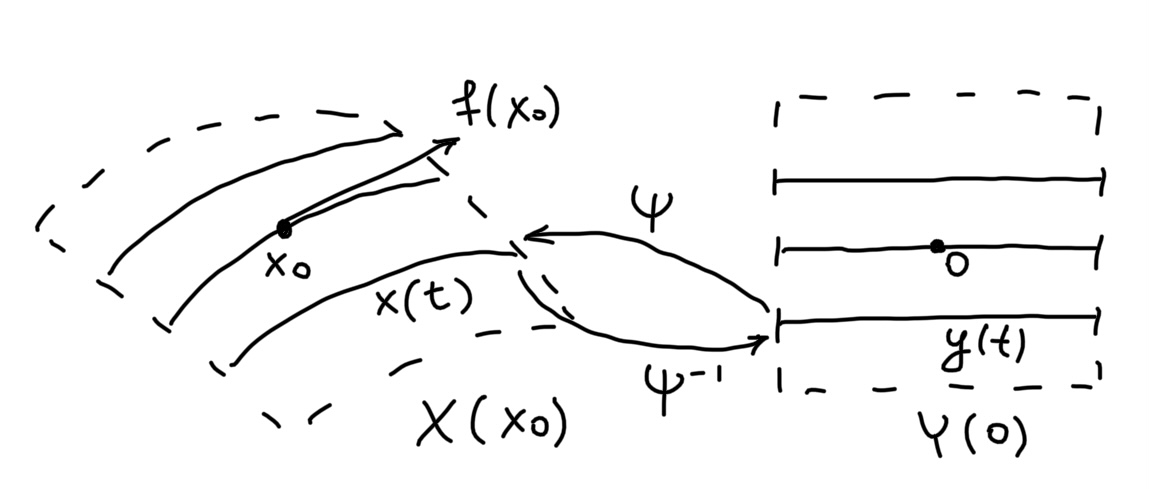
\includegraphics[scale=0.25]{trajectory-straightening}
    \centering
    \caption{Выпрямление траекторий}
\end{figure}
\begin{itemize}
    \item Говорят, что $\Psi$ выпрямляет поле направлений $f$, то есть выпрямляются не только траектории, но и касательные векторы к ним. Докажем следующую связь между $\Psi$ и $f$, которая верна в $X(x_0)$:
    \[
        \frac{\partial \Psi^{-1}}{\partial x}(x) f(x) \equiv \begin{pmatrix}
            1\\
            0\\
            \vdots \\
            0
        \end{pmatrix}.
    \]
    Возьмём какое-нибудь решение $x(t)$, тогда с одной стороны
    \[
        \frac{d \Psi^{-1}}{dt}(x(t)) \equiv \frac{\partial \Psi^{-1}}{\partial x}(x(t))x'(t) \equiv \frac{\partial \Psi^{-1}}{\partial x}(x(t))f(x(t)),
    \]
    а с другой стороны верно следующее:
    \[
        \frac{d \Psi^{-1}}{dt}(x(t)) \equiv \frac{d}{dt} \begin{pmatrix}
            t + C_1\\
            C_2\\
            \vdots\\
            C_n
        \end{pmatrix} \equiv \begin{pmatrix}
            1\\
            0\\
            \vdots\\
            0
        \end{pmatrix}.
    \]
    Ну и поскольку для любой точки $x \in X(x_0)$ можно найти решение, траектория которого проходит через $x$, то можно в равенствах везде заменить $x(t)$ на $x$.
    \item Условие $f(x_0) \ne 0$ существенно, а именно, верно следующее: если $f(x_0) = 0$, то траектории нельзя выпрямить, то есть не существует подходящих $X(x_0), \varepsilon, \Psi$ из теоремы.
    
    Действительно, точка $x_0$ является траекторией. Если бы выполнялась теорема, то в $Y(0)$ существовала бы прямая траектория, которую $\Psi$ переводил бы в $x_0$. Но тогда $\Psi$ не инъективен $\Rightarrow$ не диффеоморфизм, противоречие.
    \item Теорема носит локальный характер и обобщить её, к сожалению, нельзя. Именно, если для всех $x \in \Omega$ верно $f(x) \ne 0$, то траектории на $\Omega$ не всегда можно выпрямить. На конкретном примере примерно поймём, почему это может быть так.
    
    Возьмём систему
    \[
        \begin{cases}
            x_1' = -\cos(x_2)\\
            x_2' = \sin(x_2)
        \end{cases}.
    \]
    Её траектории выглядят как-то так:
    \begin{figure}[h]
        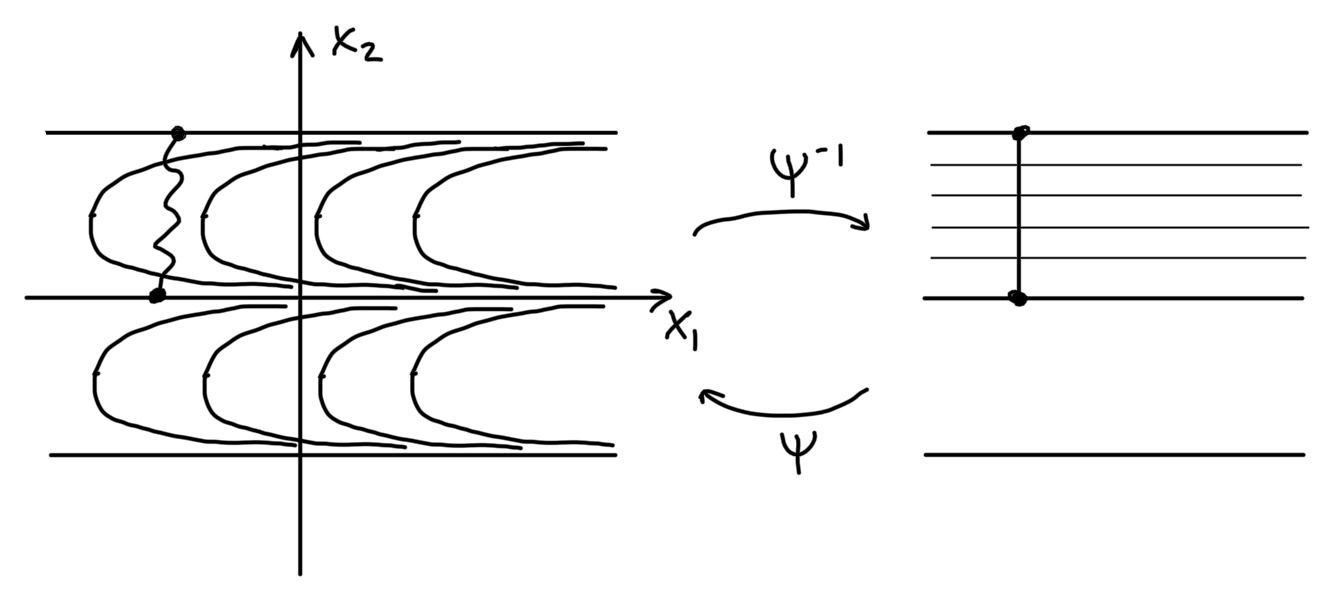
\includegraphics[scale=0.25]{arnold-example}
        \centering
        \caption{Пример Арнольда}
    \end{figure}

    Интуитивно, если бы $\Psi$ переводил прямые траектории в эти траектории, то он и отрезок между прямыми переводил бы в отрезок кривой между траекториями. Но этот отрезок между прямыми пересекает все прямые траектории, лежащие между его концами, которых бесконечно много, а
    отрезок кривой между траекториями на картинке будет пересекать лишь конечное число траекторий.
\end{itemize}

\textbf{Доказательство.} Разобьём доказательство теоремы на три этапа.
\begin{enumerate}
    \item Сначала построим отображение $\Psi$. Так как вектор $f(x_0) \ne 0$, то мы можем дополнить его $n-1$ вектором так, чтобы получился базис $(f(x_0), e_2, \dots, e_n)$ в $\mathbb R^n$. Пусть $\phi(\cdot, \xi)$ --- это непродолжаемое решение задачи Коши
    \[
        \begin{cases}
            x' = f(x)\\
            x(0) = \xi \in \Omega
        \end{cases}.
    \]
    Область определения функции $\phi$ открыта в $\mathbb R^{n+1}$ (это мы доказывали в прошлом семестре) и содержит точку $(0, x_0)$. Тогда зададим отображение $\Psi$ следующим образом: $\Psi(y) \coloneq \phi(y_1, x_0 + \sum_{i=2}^n y_ie_i)$. Область определения $\Psi$ --- это окрестность точки $0$ в $\mathbb R^n$ (так как мы можем взять близкие к нулю числа $y_1, \dots, y_n$ так, чтобы вектор $(y_1, x_0 + \sum_{i=2}^n y_ie_i)$ попал в окрестность точки $(0, x_0)$).
    Кроме того, $\phi$ непрерывно дифференцируема $\Rightarrow$ $\Psi$ тоже непрерывно дифференцируема.
    \item Теперь построим окрестности $X(x_0)$ и $Y(0)$ так, чтобы отображение $\Psi$ стало диффеоморфизмом. Для начала укажем некоторые свойства, которые нам потребуются:
    \begin{itemize}
        \item так как $\phi(\cdot, x_0)$ является решением задачи Коши, то 
        \[\left.\frac{\partial \phi}{\partial t}(t, x_0)\right|_{t=0} = \left.f(\phi(t, x_0))\right|_{t=0} = f(x_0);\]
        \item для всех $\xi \in \Omega$ верно $\phi(0, \xi) \equiv \xi$.
    \end{itemize}
    Теперь посчитаем частные производные $\Psi$. По $y_1$ она выглядит так:
    \[
        \frac{\partial \Psi}{\partial y_1}(0) = \left.\frac{\partial \phi}{\partial y_1}(y_1, x_0)\right|_{y_1=0} = f(x_0).
    \]
    При $j \geq 2$ они выглядят следующим образом:
    \[
        \frac{\partial \Psi}{\partial y_j}(0) = \left.\frac{\partial \phi}{\partial y_j}(0, x_0 + y_je_j)\right|_{y_j=0} = \left.\frac{\partial}{\partial y_j}(x_0 + y_je_j)\right|_{y_j=0} = e_j.
    \]
    Собираем всё вместе, и получаем следующую матрицу Якоби: \[\frac{\partial \Psi}{\partial y}(0) = (f(x_0) \;|\; e_2 \;|\; \dots \;|\; e_n).\]
    Теперь вспомним, что мы специально выбирали столбцы этой матрицы, чтобы они были базисом, поэтому $\rank \frac{\partial \Psi}{\partial y}(0) = n$ $\Rightarrow$ можем в нуле применить теорему об обратной функции. Из неё получаем, что существуют окрестности $X(x_0)$ и $Y(0) = (-\varepsilon, \varepsilon) \times O^{n-1}(0, \varepsilon)$ для некоторого $\varepsilon > 0$ такие, что отображение $\Psi\colon Y(0) \to X(x_0)$ является диффеоморфизмом.
    \item Теперь осталось показать, что выполняются пункты 1 и 2 из теоремы.
    Берём решение $y\colon I \to Y(0)$ системы (2), тогда \[y(t) \equiv \begin{pmatrix}
        t + C_1\\
        C_2\\
        \vdots\\
        C_n
    \end{pmatrix}.\]
    Применим к нему отображение $\Psi$:
    \[
        x(t) \coloneq \Psi(y(t)) \equiv \phi(t + C_1, x_0 + \sum_{j=2}^n C_je_j).
    \]
    Так как в автономных системах сдвиг по $t$ не влияет на свойство «быть решением», то $x(t)$ является решением системы (1) $\Rightarrow$ первый пункт выполняется.

    Теперь покажем, что второй пункт тоже верен. К сожалению, технически это будет довольно неприятно. Берём решение $x\colon I \to X(x_0)$ системы (1). Хотим показать, что функция $\Psi^{-1}(x(t))$ является решением системы (2). Пусть $t^* \in I$ и \[y^* \coloneq \Psi^{-1}(x(t^*)) = \begin{pmatrix}
        y_1^*\\
        \vdots\\
        y_n^*
    \end{pmatrix}.\]
    Через точку $y^*$ проходит траектория какого-то решения $y(t)$, тогда оно должно выглядеть как-то так:
    \[
        y(t) \coloneq \begin{pmatrix}
            t + y_1^* -t^*\\
            y_2^*\\
            \vdots\\
            y_n^*
        \end{pmatrix}.
    \]
    Первая координата так странно выглядит, так как мы хотим, чтобы она попадала в $\varepsilon$-окрестность нуля. Это будет так, если $t \in I^* \coloneq (-\varepsilon + t^* - y_1^*, \varepsilon + t^* - y_1^*)$. Подействуем теперь на эту траекторию отображением $\Psi$, тогда по уже доказанному первому пункту она перейдёт в какую-то траекторию решения системы (1). Нам нужно, чтобы эта траектория совпала с траекторией решения $x(t)$.

    Распишем, куда переходит при действии $\Psi$ точка $y(t^*)$:
    \[
        \Psi(y(t^*)) = \Psi(y^*) = \Psi(\Psi^{-1}(x(t^*))) = x(t^*).
    \]
    Получили, что в точке $t^*$ решения $x(t)$ и $\Psi(y(t))$ совпадают, но тогда по теореме о существовании и единственности решения получаем, что $\Psi(y(t)) \equiv x(t) \Leftrightarrow y(t) \equiv \Psi^{-1}(x(t))$ при $t \in I \cap I^*$. Это почти то, что нам нужно, только мы хотим, чтобы это тождество выполнялось на всём $I$. Докажем, что на самом деле $I \subset I^*$.

    Пусть $I \nsubseteq I^*$. Тогда либо $\sup I^* \in I$, либо $\inf I^* \in I$. Без ограничения общности рассмотрим первый случай. Возьмём последовательность $\{t_n\} \subset I^*$, сходящуюся к $\sup I^*$. Поймём, куда сходится $y(t_n)$. Первая координата этого вектора, согласно тому, как мы задавали функцию $y$, равна $t_n + y_1^* - t^* \to \sup I^* + y_1^* - t^*$. По построению интервала $I^*$ следует, что $\sup I^* = \varepsilon + t^* - y_1^*$. Тогда первая координата сходится к $\varepsilon$ $\Rightarrow$ $\lim_{n\to\infty}y(t_n) \notin Y(0)$, так первая координата попала на границу окрестности $(-\varepsilon, \varepsilon)$.
    С другой стороны $y(t_n) = \Psi^{-1}(x(t_n))$. Так как композиция непрерывных функций непрерывна, получаем, что $y(t_n) \to \Psi^{-1}(x(\sup I^*)) \in Y(0)$. Получили противоречие.
\end{enumerate}

\QED

% \textbf{Замечание.} Эту лемму можно использовать для доказательства фактов про первые интегралы, ибо у системы (4) есть $n - 1$ независимый первый интеграл --- проекции на $y_1, \dots, y_{n-1}$.

\setcounter{equation}{0}
\section{Устойчивость по Ляпунову и асимптотическая устойчивость}
\subsection{Определение и примеры}
Снова заданы открытое множество $\Omega \subset \mathbb R^n$, отображение $f \in C^1(\Omega, \mathbb R^n)$, положение равновесия $\widehat{x} \in \Omega$ и автономная система
\begin{equation}
    x' = f(x).
\end{equation}
Пусть $\phi(\cdot, \xi)$ --- непродолжаемое решение задачи Коши 
\[
\begin{cases}
    x' = f(x)\\
    x(0) = \xi
\end{cases}.
\]
\textbf{Определение.} Положение равновесия $\widehat{x}$ называется \textit{устойчивым по Ляпунову}, если:
\begin{enumerate}
    \item cуществует $r > 0$ такое, что для любого $\xi \in O(\widehat{x}, r)$ отображение $\phi(\cdot, \xi)$ определено на $[0, +\infty)$;
    \item для любого $\varepsilon > 0$ существует $\delta > 0$ такое, что для всех $\xi \in O(\widehat{x}, \delta)$ и для всех $t \in [0, +\infty)$ верно $\phi(t, \xi) \in O(\widehat{x}, \varepsilon)$.
\end{enumerate}

\textbf{Определение.} Положение равновесия $\widehat{x}$ называется \textit{асимптотически устойчивым}, если:
\begin{enumerate}
    \item оно устойчиво по Ляпунову;
    \item cуществует $d > 0$ такое, что для всех $\xi \in O(\widehat{x}, d)$ функция $\phi(t, \xi) \to \widehat{x}$ при $t \to +\infty$.
\end{enumerate}

\textbf{Примеры.} 
\begin{itemize}
    \item Пусть $\Omega \subset \mathbb R$ и $\widehat{x}$ --- изолированное положение равновесия, то есть существует окрестность $\widehat{x}$ такая, что в ней нет других положений равновесия.
        Тогда один из возможных случаев: это когда в этой окрестности функция $f \geq 0$ и равна нулю только в точке $\widehat{x}$.
        
        Посмотрим на интегральные кривые. Есть горизонтальная прямая, соответствующая решению
        $x(t) \equiv \widehat{x}$. Если берём начальное условие $\xi < \widehat{x}$, то соответствующее решение будет монотонно возрастать в силу положительности производной, тогда из теоремы о существовании и единственности следует, что горизонтальная прямая будет его асимптотой. Если же берём начальное условие выше $\widehat{x}$, то решение снова будет возрастать. Тогда здесь нет даже устойчивости по Ляпунову.
        А вот если рассмотреть случай, когда функция $f(x) > 0$ при $x < \widehat{x}$ и $f(x) < 0$ при $x > \widehat{x}$, то аналогичным образом можно показать, что там будет асимптотическая устойчивость, а тогда и устойчивость по Ляпунову.
    \item Пусть теперь $\Omega \subset \mathbb{R}^2$, $f(x) = Ax$ и $\widehat{x} = 0$. Возвращаясь к случаям из предыдущего параграфа, устойчивость по Ляпунову будет на всех устойчивых портретах, а ещё для центра. Они же, но уже за исключением центра, будут и асимптотически устойчивы.
    
\end{itemize}
\subsection{Достаточные условия устойчивости}
\subsubsection{Устойчивость линейных систем}
Пусть даны матрица $A \in \mathbb R^{n \times n}$ и система
\begin{equation}
    x' = Ax.
\end{equation}
% Пусть $X(t)$ --- фундаментальная система решений системы (2), такая что $X(0) = I$ (единичная).
% Она существует, так как можно рассмотреть $n$ задач Коши $x' = Ax$ и $x(0) = e_i$, где $e_i$ --- $i$-ый базисный вектор $\mathbb R^n$.
Пусть в ЖНФ матрицы $A$ есть жордановы клетки $K_1, \dots, K_m$, причём для каждой клетки $K_j$ её размер равен $k_j$ и ей соответствует собственное число $\lambda_j = \alpha_j + i\beta_j$. Без ограничения общности будем считать, что $\lambda_1, \dots, \lambda_s \in \mathbb C$, при этом им соответствуют сопряжённые числа $\lambda_{s+1} = \overline{\lambda_1}, \dots, \lambda_{2s} = \overline{\lambda_s}$, а $\lambda_{2s+1}, \dots, \lambda_m \in \mathbb R$.

\textbf{Теорема.} 
\begin{enumerate}
    \item Если все $\re(\lambda_j) < 0$, то $\widehat{x} = 0$ --- асимптотически устойчивое положение равновесия.
    \item Если все $\re(\lambda_j) \le 0$, а для $j$ таких, что $\re(\lambda_j) = 0$, выполнено $k_j = 1$, то $\widehat{x} = 0$ устойчиво по Ляпунову, но не асимптотически устойчиво.
    \item В остальных случаях $\widehat{x} = 0$ не устойчиво по Ляпунову.
\end{enumerate}

\textbf{Доказательство.} Из прошлого семестра мы знаем, что любое решение $x(t)$ системы (2) представимо в виде
\[
    x(t) = \sum_{j=1}^{s} P_j(t) e^{\alpha_j t}\cos(\beta_j t) + \sum_{j=s+1}^{2s} P_j(t) e^{\alpha_{j-s} t}\sin(\beta_{j-s} t) + \sum_{j=2s+1}^{m} P_j(t) e^{\lambda_j t},
\]
причём $\deg P_j \le k_j - 1$.

\begin{enumerate}
\item Из условия $\re \lambda_j < 0$ следует, что $|x(t)| \to 0$ при $t \to +\infty$. Пусть $X(t)$ --- ФМР. Так как столбцы $X(t)$ являются решениями, $\|X(t)\| \to 0$ при $t \to +\infty$.
Тогда $\|X(t)\|$ равномерно ограничена некоторым числом $c > 0$. Кроме того, имеем следующее неравенство:
\[
    |\phi(t, \xi)| = |X(t) \xi| \le \| X(t) \| \cdot |\xi|.
\]
Заметим, что $\phi(\cdot, \xi)$ при любом $\xi$ определено на $[0, +\infty)$, так как (2) является линейной системой с постоянными коэффициентами. Зафиксируем $\varepsilon > 0$. Чтобы выполнялся второй пункт из определения устойчивости по Ляпунову, можно взять $\delta = \frac{\varepsilon}{2c}$, тогда
при $\xi \in O(0, \delta)$ из неравенства выше получаем, что 
\[
    |\phi(t, \xi)| \leq c \cdot \frac{\varepsilon}{2c} = \frac{\varepsilon}{2} < \varepsilon.
\]
Асимптотическая устойчивость следует из того, что $\|X(t)\| \to 0$, а $|\xi|$ ограничен.

\item Если $\re(\lambda_j) < 0$, то соответствующее слагаемое стремится к нулю $\Rightarrow$ ограничено на $[0, +\infty)$.
Остаётся случай $\re(\lambda_j) = 0 \Rightarrow k_j = 1$. Тут мы пользуемся тем, что $\deg P_j(t) \le 1 - 1 = 0$ $\Rightarrow$ многочлен $P_j$ --- это просто константа. Тогда и всё соответствующее слагаемое будет ограничено.
Значит, каждое решение $x(t)$ на $[0, +\infty)$ ограничено, тогда существует такое число $c > 0$, что $\|X(t)\| \le c$ для всех $t \in [0, +\infty)$. Далее работает такое же рассуждение, как в первой части, поэтому получаем устойчивость по Ляпунову. Вывод об асимптотической устойчивости мы так сразу сделать не можем, так как не все решения стремятся к нулю. Покажем, что здесь её просто не может быть, предъявив явное решение.

Пусть $j$ таково, что $\re \lambda_j = 0, k_j = 1$. Тогда если $\lambda_j \in \mathbb C$, то берём решение $x(t) \coloneq r(v_j \cos(\beta_j t) + u_j\sin(\beta_j t))$, где $r > 0$, $u_j, v_j \in \mathbb R^n$. Уменьшая $r$, мы можем попасть в сколь угодно малую окрестность нуля, но при этом $x(t) \nrightarrow 0$. Если же $\lambda_j \in \mathbb R$, то возьмём решение $x(t) \coloneq rv_j$. Оно опять же не стремится к нулю.

\item Пусть существует $j$ такое, что $Re(\lambda_j) > 0$. Если $\lambda_j \in \mathbb C$, то берём решение $x(t) \coloneq re^{\alpha_j t} (P_j(t)\cos(\beta_j t) + P_{j+s}(t)\sin(\beta_j t))$. Для любого $r > 0$ оно не ограничено $\Rightarrow$ нет устойчивости по Ляпунову.
Если же $\lambda_j \in \mathbb R$, то подойдёт решение $x(t) \coloneq r e^{\lambda_j t}v_j$, $r > 0$, $v_j \in \mathbb R^n$.

Остался случай, когда все $\re \lambda_j \le 0$ и существует $j$ такое, что $\re \lambda_j = 0$, но при этом $k_j \ge 2$. Тогда если $\lambda_j \in \mathbb C$, то есть неограниченное комплексное решение $x(t) \coloneq r(a+bt)e^{\lambda_jt}$, $r > 0$, $b \ne 0$. Тогда либо $\re x(t)$, либо $\im x(t)$ не ограничено $\Rightarrow$ нет устойчивости по Ляпунову.
Если же $\lambda_j \in \mathbb R$, то возьмём решение $x(t) \coloneq r(at + b)$, $a, b \in \mathbb R^n$, $a \ne 0$, $r > 0$. Снова $x(t)$ не ограничено $\Rightarrow$ нулевое положение равновесия не устойчиво по Ляпунову.
\end{enumerate}

\QED

% \subsubsection{Устойчивость нелинейных систем}
% Пусть $\Omega \subset \mathbb{R}^n$ открыто, $f \in C^1(\Omega, \mathbb{R}^n)$, $\widehat{x} \in \Omega$ --- положение равновесия.
% Рассмотрим задачу Коши
% \[
% \begin{cases}
%     x' = f(x)\\
%     x(0) = x_0
% \end{cases}.
% \]
% Пусть $\phi(\cdot, x_0)$ --- её непродолжаемое решение. Обозначим матрицу Якоби $A \coloneq \frac{\partial f}{\partial x}(\widehat{x})$. Пусть $\lambda_1, \dots, \lambda_k$ --- собственные числа матрицы $A$.

% \textbf{Теорема.} (Ляпунова) Если все $\re \lambda_j < 0$, то положение равновесия $\widehat{x}$ асимптотически устойчиво.

% \textbf{Замечания.}
% \begin{enumerate}
%   \item Помним, что можно разложить функцию по формуле Тейлора:
%   \[
%   f(x) \equiv A(x- \widehat{x}) + r(x-\widehat{x}),
%   \]
%   при этом $r(x-\widehat{x}) = o(|x-\widehat{x}|)$ при $|x-\widehat{x}| \to 0$.
% \item Вспомним лемму о дифференциальном неравенстве. Она гласит, что если нам дан интервал $I \subset \mathbb{R}$, $t_0 \in I$, $z \in C^1(I, \mathbb{R}^n)$, $A > 0$, $B \ge 0$,
% а также на всём $I$ выполнено неравенство $|z'(t)| \le A|z(t)| + B$, то верно следующее неравенство:
% \[
%   |z(t)| \le |z(t_0)|e^{A(t-t_0)} + \frac{B}{A}(e^{A(t-t_0)} - 1).
% \]
% Нам оно нужно в частном случае, когда $t_0 = 0$. Сделаем следующее: подставим это неравенство в неравенство из условия леммы, получим следующее:
% \[
%   |z'(t)| \le A|z(0)|e^{At} + Be^{At}.
% \]

% \end{enumerate}

% Рассмотрим систему
% \begin{equation}
%     x' = f(x).
% \end{equation}

% \textbf{Определение.} Пусть $\Pi \subset \Omega$ открыто, а функция $v \in C^1(\Pi, \mathbb{R})$. Тогда \textit{производной в силу системы (1)} называется функция
% \[
%   \left.\frac{dv}{dt}\right|_{(1)}(x) \coloneq \left< \frac{\partial v}{\partial x}(x), f(x) \right> = \sum_{j=1}^n{\frac{\partial v}{\partial x_j}(x)f_j(x)}.
% \]
% Пусть $x(t)$ --- решение системы (1). Тогда
% \[
%     \frac{dv}{dt}(x(t)) \equiv \left< \frac{\partial v}{\partial x}(x(t)), x'(t) \right> \equiv \left< \frac{\partial v}{\partial x}(x(t)), f(x(t)) \right> \equiv \left.\frac{dv}{dt}\right|_{(1)}(x(t)).
% \]

% \textbf{Определение.} Функция $v$ в следующих двух теоремах называется \textit{функцией Ляпунова}.

% \textbf{Теорема.} (Ляпунова об устойчивости) Пусть существуют $\varepsilon > 0$ и функция $v \in C^1(O(\widehat{x}, \varepsilon), \mathbb R)$ такие, что:
% \begin{enumerate}
%   \item $v(\widehat{x}) = 0$
%   \item $v(x) > 0$ при $x \ne \widehat{x}$
%   \item для всех $x$ выполнено $\left.\frac{dv}{dt}\right|_{(1)}(x) \le 0$.
% \end{enumerate}
% Тогда $\widehat{x}$ устойчиво по Ляпунову.

% \textbf{Теорема.} (Ляпунова об асимптотической устойчивости) Пусть существуют $\varepsilon > 0$ и функция $v \in C^1(O(\widehat{x}, \varepsilon), \mathbb R)$ такие, что:
% \begin{enumerate}
%   \item выполнены условия 1 и 2 из предыдущей теоремы
%   \item для всех $x \ne \widehat{x}$ выполнено $\left.\frac{dv}{dt}\right|_{(1)}(x) < 0$.
% \end{enumerate}
% Тогда $\widehat{x}$ асимптотически устойчиво.

% \textbf{Примеры.}
% \begin{itemize}
%   \item Рассмотрим уравнение $x' = -x^3$, $\widehat{x} = 0$. Тогда в качестве функции Ляпунова можно взять $v(x) = x^2$. Тогда для $x \ne 0$ верно следующее:
%   \[
%     \left.\frac{dv}{dv}\right|_{(1)}(x) = 2x \cdot (-x^3) = -2x^4 < 0.
%   \]
%   Получаем, что выполнены все три условия теоремы Ляпунова об асимптотической устойчивости $\Rightarrow$ $\widehat{x} = 0$ асимптотически устойчиво.
%   \item Рассмотрим систему 
%   \[
%       \begin{cases}
%           x_1' = -x_2 \\
%           x_2' = x_1
%       \end{cases}
%   \]
%   и $\widehat{x} = (0, 0)^T$.
%   Положим $v(x) = x_1^2 + x_2^2$. Тогда $v(0) = 0$ и $v(x) > 0$ при $x \ne 0$.
%   Найдём производную:
%   \[
%       \left.\frac{dv}{dt}\right|_{(1)} (x) = \left< (2x_1, 2x_2)^T, (-x_2, x_1)^T \right> \equiv 0.
%   \]
%   Следовательно, по теореме Ляпунова об устойчивости $\widehat{x}$ устойчиво.
%   Но асимптотической устойчивости нет, так как фазовым портретом этой системы является центр.
% \end{itemize}

\setcounter{equation}{0}
\section{Первые интегралы}
\subsection{Первые интегралы автономных систем}
Пусть $\Omega \subset \mathbb R^{n}$ открыто и $f \in C^1(\Omega, \mathbb R^n)$. Снова рассматриваем автономную систему
\begin{equation}
    x' = f(x).
\end{equation}

\textbf{Определение.} Если $D \subset \Omega$ открыто, то \textit{первым интегралом} системы (1) называется непрерывно дифференцируемая функция $u\colon D \to \mathbb R$ такая, что $u(x(t)) \equiv$ const для любого такого решения $x\colon I \to \mathbb{R}$ системы (1), что $x(I) \subset D$.

\textbf{Замечание.} Первый интеграл всегда существует, например, $u \equiv$ const.

\textbf{Утверждение.} (критерий первого интеграла) Пусть $D \subset \Omega$ открыто и функция $u\colon D \to \mathbb R$ непрерывно дифференцируема. Тогда $u(\cdot)$ --- первый интеграл системы (1) $\Leftrightarrow$ $\left.\frac{du}{dt}\right|_{(1)}(x) \equiv 0$.

\textbf{Доказательство.} $\Rightarrow$: Берём $x_0 \in D$. Тогда существует решение $x\colon I \to \mathbb{R}^n$ задачи Коши
\[
    \begin{cases}
        x' = f(x) \\
        x(t_0) = x_0
    \end{cases}
\]
для некоторого $t_0 \in I$. При этом при необходимости можно сузить область определения $I$ так, чтобы $x(I) \subset D$.
Так как функция $u(x(t)) \equiv$ const, то по свойству производной в силу системы
\[
    \left.\frac{du}{dt}\right|_{(1)}(x(t)) \equiv \frac{du}{dt}(x(t)) \equiv 0.
\]
Подставляем $t = t_0$, получаем: $\left.\frac{du}{dt}\right|_{(1)}(x_0) = 0$. В силу произвольности выбора $x_0$ получили требуемое.

$\Leftarrow$: Берём произвольное решение $x\colon I \to \mathbb{R}$ системы (1) такое, что $x(I) \subset D$. Тогда
\[
\frac{du}{dt}(x(t)) \equiv \left.\frac{du}{dt}\right|_{(1)}(x(t)) \equiv 0,
\]
отсюда получаем, что $u(x(t)) \equiv$ const $\Rightarrow$ по определению $u(\cdot)$ --- первый интеграл системы (1).

\QED

\textbf{Примеры.}
\begin{itemize}
    \item Пусть $\Omega = \mathbb{R}^2$, $D = \mathbb{R}^2$. Рассмотрим систему $x' = x$. Её решение --- это $x_1=c_1e^t$, $x_2=c_2e^t$.
    На фазовом портрете траекториями будут все открытые лучи, выходящие из начала координат. Пусть $u(\cdot)$ --- первый интеграл. Возьмём конкретный луч, на нём $u \equiv c$ для какой-то константы $c$.
    По непрерывности $u(0) \equiv c$. Но тогда на всех лучах $u \equiv c$, значит, $u \equiv c$ на всём $D$ и других первых интегралов быть не может.
    \item Рассмотрим ту же самую систему, только теперь $D = \{(x_1, x_2)^T : x_1 > 0\}$. Покажем, что функция $u(x) = \frac{x_2}{x_1}$ является первым интегралом. Действительно,
    \[
        u(x(t)) \equiv \frac{c_2e^t}{c_1e^t} \equiv \frac{c_2}{c_1}.
    \]
    \item Рассмотрим систему
    \[
        \begin{cases}
            x_1' = -x_2 \\
            x_2' = x_1
        \end{cases}.
    \]
    Её решение выглядит так:
    \[
        \begin{cases}
            x_1 = r\cos(\phi+t)\\
            x_2 = r\sin(\phi+t)
        \end{cases}.
    \]
    Тогда на фазовом портрете траекториями будут концентрические окружности. Так как при движении точки по окружности радиус не зависит от $t$, то в качестве первого интеграла можно взять $u(x) = x_1^2 + x_2^2$.
    % Так как $f(x_0) = (0, 0)$, предположение теоремы нарушается.
    % Проверим, что следствие теоремы тоже нарушится: от противного, пусть существует первый интеграл $v(x_1, x_2)$ в окрестности $x_0$.
    % Мы ещё требуем невырожденность, поэтому
    % \[
    %     \left( \frac{\partial v}{\partial x_1}(0, 0), \frac{\partial v}{\partial x_2}(0, 0) \right) \ne (0, 0).
    % \]
    % Без ограничения общности $\frac{\partial v}{\partial x_1}(0, 0) > 0$, тогда это верно и в некоторой окрестности нуля.
    % По определению первого интеграла производная в силу системы должна быть тождественным нулём:
    % \[
    %     -x_2 \frac{\partial v}{\partial x_1}(x_1, x_2) + x_1 \frac{\partial v}{\partial x_2}(x_1, x_2) \equiv 0.
    % \]
    % Возьмём $x_1 = 0$ и $x_2 = \frac{1}{N}$, где $N$ --- какое-то достаточно большое число.
    % Тогда из доказанного выше $\frac{\partial v}{\partial x_1}(x_1, x_2) > 0$.
    % Вернёмся к тождеству выше:
    % \[
    %     -x_2 \frac{\partial v}{\partial x_1}(x_1, x_2) \equiv 0.
    % \]
    % Но мы взяли $x_1$, $x_2$ так, что оба множителя не равны нулю --- противоречие.

    % \QED
\end{itemize}

\textbf{Замечание.} Зачем нужны первые интегралы? Оказывается, с помощью них можно сводить автономные системы к алгебраическим уравнениям. Нестрого поясним, как это можно делать. Пусть $\Omega \subset \mathbb{R}^3$.
Возьмём два первых интеграла $u_1, u_2$, константы $c_1, c_2$ и рассмотрим следующую систему:
\[
    \begin{cases}
        u_1(x) = c_1\\
        u_2(x) = c_2
    \end{cases}.
\]
Оба уравнения задают поверхности, а решения системы составляют кривую, по которой пересекаются эти поверхности. Можно показать, что кусочки этой кривой будут являться траекториями автономной системы.

\textbf{Определение.} Пусть $D \subset \Omega$ открыто и функции $v_1, \dots, v_k \in C^1(D, \mathbb{R}), k < n$.
Тогда они называются \textit{функционально независимыми} на $D$, если ранг матрицы Якоби $\rank \frac{\partial(v_1, \dots, v_k)}{\partial(x_1, \dots, x_n)} \equiv k$.

\textbf{Замечание.} Из функциональной независимости следует линейная независимость, а вот обратное следствие неверно. Например, пусть $D = \mathbb{R}^2$. Возьмём $u(x_1, x_2) = x_1^2$. Заметим, что при $x_1 = 0$ ранг матрицы Якоби равен $0 < 1$, значит, нет функциональной независимости.

% \textbf{Теорема.} Для любой точки $(t_0, x_0) \in \Omega$ существует окрестность $D \subset \Omega$, а в ней --- независимые в $D$ первые интегралы $v_1, \dots, v_n$.

% \textbf{Доказательство.} Для любого $(t_0, \xi) \in D$ существует единственное непродолжаемое решение $\phi(\cdot, \xi)$ задачи Коши, ещё и непрерывно дифференцируемое:
% \[
%     \begin{cases}
%         x' = f(t, x) \\
%         x(t_0) = \xi 
%     \end{cases} .
% \]
% Решим уравнение $x - \phi(t, \xi) = 0$ относительно $\xi$ с параметрами $(t, x)$ в окрестности $(t_0, x_0)$, соответствующей решению $x = x_0$, $t = t_0$, $\xi = x_0$.
% Тогда $\phi(t_0, \xi) \equiv \xi$ по определению $\phi$.
% Теперь
% \[
%     \frac{\partial}{\partial \xi} (x - \phi(t, \xi)) \bigg|_{\substack{t = t_0 \\ x = x_0}}(x_0) = -E.
% \]
% ($x_0$ встречается дважды, так как сначала мы подставили параметр $x = x_0$, а потом неизвестную $\xi = x_0$)

% Следовательно, применима теорема о неявной функции: существует окрестность $D_1 \subset \Omega$ точки $(t_0, x_0)$ и отображение $V = (v_1, \dots, v_n): D_1 \to \mathbb R^n$, такое что:
% \begin{itemize}
%     \item $V \in C^1$.
%     \item Для всех $(t, x) \in D_1$ выполнено $x - \phi(t, V(t, x)) \equiv 0$.
%     \item $V(t_0, x_0) = x_0$.
%     \item Так как количество уравнений совпадает с количеством неизвестных, существует окрестность $\Delta$ точки $x_0$, такая что если $u \in \Delta$ и $x - \phi(t, u) = 0$, то $u = V(t, x)$.
% \end{itemize}
% Продифференцируем по $x$ второе свойство:
% \[
%     E \equiv \frac{\partial \phi}{\partial \xi}(t, V(t, x)) \cdot \frac{\partial V}{\partial x}(t, x).
% \]
% Подставим $(t_0, x_0)$: заметим, что $V(t_0, x_0) = x_0$, откуда это будет равно
% \[
%     E = \frac{\partial \phi}{\partial \xi}(t_0, x_0) \cdot \frac{\partial V}{\partial x}(t_0, x_0).
% \]
% Первый множитель равен $E$, поэтому
% \[
%     E = \frac{\partial V}{\partial x}(t_0, x_0).
% \]
% Отсюда ранг этой матрицы равен $n$, а значит, существует окрестность $D \subset D_1$, такая что в ней $\rank \left( \frac{\partial V}{\partial x} (t, x) \right) = n$.

% Пусть $x(\cdot)$ --- решение задачи Коши $x' = f(t, x)$, $x(t_0) = \xi$.
% По второму свойству $x(t) - \phi(t, V(t, x(t))) \equiv 0$.
% Более того, из обозначений $x(t) - \phi(t, \xi) \equiv 0$.
% Уменьшая область определения $x(\cdot)$, можно добиться того, чтобы $x(t)$ всегда попадал в $\Delta$, откуда по четвёртому свойству решение единственно и должно совпадать, поэтому $V(t, x(t)) \equiv \xi$, то есть $v_i(t, x(t)) \equiv \xi_i$ --- константы.

% \QED

% \subsection{Первые интегралы автономных систем}
% Пусть нам даны $n \in \mathbb N$, открытое $\Omega \subset \mathbb R^n$ и отображение $f: \Omega \to \mathbb R^n$, $f \in C^1$.
% Рассмотрим систему
% \begin{equation}
%     x' = f(x).
% \end{equation}

% \textbf{Теорема.} Для любого $x_0 \in \Omega$, такого что $f(x_0) \ne 0$ существует окрестность $D \subset \Omega$ точки $x_0$ и $n - 1$ независимых первых интегралов $v_i: D \to \mathbb R$.
% От предыдущего случая отличается тем, что $v_i$ не зависит от $t$.

% \textbf{Доказательство.}
% Так как $f(x_0) \ne 0$, у него существует ненулевая координата.
% Без ограничения общности это $n$-ая: $f_n(x_0) \ne 0$.
% Из непрерывности $f_n$ получаем, что $f_n(x) \ne 0$ в некоторой окрестности $x_0$.
% Рассмотрим неавтономную систему
% \begin{equation}
%     \frac{dx_i}{dx_n} = \frac{f_i(x)}{f_n(x)}.
% \end{equation}
% Здесь $(n - 1)$ уравнение, откуда по теореме из предыдущего пункта существует окрестность $D$ точки $x_0$ и независимые первые интегралы системы (3) $v_1, \dots, v_{n-1}: D \to \mathbb R$.

% Пусть $\phi(\cdot) = (\phi_1(\cdot), \dots, \phi_n(\cdot))$ --- какое-то решение системы (2), такое что для всех $t$ $\phi(t) \in D$, то есть $\phi_n'(t) = f_n(\phi(t)) \ne 0$
% Итак, мы получили строго монотонную функцию $\phi_n(t)$ на интервале --- по первому семестру матанализа существует обратная к ней функция $t(\phi_n)$.
% Обозначим $x_i(x_n) = \phi_i(t(x_n))$.
% Тогда
% \[
%     \frac{dx_i}{dx_n}(x_n) \equiv \frac{d \phi_i}{dt}(t(x_n)) \cdot \frac{dt}{dx_n}(x_n) \equiv f_i(\phi(t(x_n))) \cdot \frac{1}{\phi_n'(t(x_n))} \equiv
% \]
% \[
%     \equiv \frac{f_i(\phi(t(x_n)))}{f_n(\phi(t(x_n)))} \equiv \frac{f_i(x)}{f_n(x)}.
% \]
% Вернёмся к первым интегралам: по определению для всех $i$
% \[
%     v_i(\phi_1(t(x_n)), \dots, \phi_{n-1}(t(x_n)), x_n) \equiv const.
% \]
% Обозначая $\tau = t(x_n)$, получаем
% \[
%     v_i(\phi_1(\tau), \dots, \phi_n(\tau)) \equiv const.
% \]
% Значит, $v_i$ являются первыми интегралами системы (2).
% Проверим их независимость.
% Мы знаем, что они независимы в системе (3), тогда векторы
% \[
%     \left(\frac{\partial v_i}{\partial x_1}(x), \dots, \frac{\partial v_i}{\partial x_{n-1}}(x) \right)
% \]
% линейно независимы.
% Нам нужны $n$-мерные векторы, поэтому добавим к ним ещё одну координату:
% \[
%     \left(\frac{\partial v_i}{\partial x_1}(x), \dots, \frac{\partial v_i}{\partial x_{n-1}}(x), \frac{\partial v_i}{\partial x_n}(x) \right).
% \]
% При добавлении новой координаты линейная независимость не ломается, поэтому они подходят в систему (2).
% Таким образом, ранг матрицы 
% \[
%     \left( \frac{\partial v_i}{\partial x_j} \right)_{\substack{i = \overline {1, n - 1} \\ j = 1, n}}
% \]
% равен $n - 1$, то есть $v_1, \dots, v_{n-1}$ --- искомые первые интегралы.

% \QED

% \textbf{Замечание.} Зачем: возьмём $n = 2$ и первый интеграл $v_1$.
% Тогда кривая $v_1(x) = v_1(x_0)$ является фазовой траекторией.
% Аналогично в трёхмерном случае, но тогда будет пересечение поверхностей.

% \textbf{Пример.} Рассмотрим систему

\subsection{Множество всех первых интегралов автономной системы}
\textbf{Утверждение.} Если у нас есть $k$ первых интегралов $u_1(x), \dots, u_k(x)$ системы (1), то функция $F(u_1(x), \dots, u_k(x))$, где $F$ непрерывно дифференцируема, также является первым интегралом системы (1).

\textbf{Доказательство.} Действительно, пусть $x(t)$ --- это решение системы (1), тогда
\[
    F(u_1(x(t)), \dots, u_k(x(t))) \equiv F(\text{const}, \dots, \text{const}) \equiv \text{const}.
\]

\QED

Поскольку первых интегралов бесконечное количество (хотя бы потому, что все константы ими являются), то возникает вопрос: можно ли взять несколько первых интегралов и, используя утверждение выше, получить все возможные первые интегралы? Оказывается, что при определённых условиях так правда можно сделать.

\textbf{Теорема.} Пусть $x_0 \in \Omega$ и $f(x_0) \ne 0$. Тогда существуют окрестность $X(x_0)$ и $n-1$ функционально независимых первых интегралов $u_2, \dots, u_{n}\colon X(x_0) \to \mathbb{R}$ системы (1).

\textbf{Доказательство.} Докажем теорему для случая, когда у нас фазовые траектории являются прямыми, а потом сведём общий случай к этому с помощью теоремы о выпрямлении траекторий. Давайте всё формализуем.
\begin{enumerate}
    \item Так как $f(x_0) \ne 0$, то мы можем использовать теорему о выпрямлении траекторий. Значит, существует окрестности $X(x_0)$, $Y(0)$ и диффеоморфизм $\Psi\colon Y(0) \to X(x_0)$. Зададим для $i=\overline{2, n}$ функции $v_i\colon Y(0) \to \mathbb{R}$ по формуле $v_i(y) \coloneq y_i$.
    Тогда все $v_i$ --- это первые интегралы системы
    \begin{equation}
        \begin{cases}
            y_1' = 1\\
            y_2' = 0\\
            \vdots\\
            y_n' = 0
        \end{cases},
    \end{equation}
    так как любое решение этой системы имеет вид
    \[
        y(t) = \begin{pmatrix}
            t+C_1\\
            C_2\\
            \vdots\\
            C_n
        \end{pmatrix},
    \]
    а тогда $v_i(y(t)) \equiv c_i$. При этом все $v_i$ функционально независимы в окрестности $Y(0)$, так как $\grad v_i(y(t)) = (0, \dots, 1, \dots, 0)^T$, где $1$ стоит на месте $i$, тогда у матрицы Якоби как раз будет ранг $n-1$.
    \item Теперь введём функции $u_2, \dots, u_n\colon X(x_0) \to \mathbb{R}$ по формуле $u_i(x) \coloneq v_i(\Psi^{-1}(x))$. Тогда все $u_i$ --- это первые интегралы системы (1), так как для любого решения $x(t)$ системы (1) $\Psi^{-1}(x(t))$ будет решением системы (2), а тогда
    \[
        u_i(x(t)) \equiv v_i(\Psi^{-1}(x(t))) \equiv \text{const}.
    \]
    Ну и все $u_i$ функционально независимы на $X(x_0)$, так как $v_i$ функционально независимы, а $\Psi$ --- это диффеоморфизм $\Rightarrow$ его матрица Якоби невырожденная и при домножении на невырожденную матрицу ранг не меняется.

    \QED
\end{enumerate}


\textbf{Теорема.} Пусть $x_0 \in \Omega$ и $f(x_0) \ne 0$. Тогда для любых функционально независимых первых интегралов $u_1, \dots, u_{n-1}\colon X(x_0) \to \mathbb{R}$ системы (1) существуют окрестности $X'(x_0) \subset X(x_0)$ и $W((u_1(x_0), \dots, u_{n-1}(x_0)))$ такие, что
для любого первого интеграла $u\colon X'(x_0) \to \mathbb{R}$ системы (1) существует функция $F \in C^1(W, \mathbb{R})$: $u(x) \equiv F(u_1(x), \dots, u_{n-1}(x))$.

\textbf{Доказательство.} Здесь мы снова докажем теорему сначала для системы (2), а потом перенесём всё на систему (1) с помощью теоремы о выпрямлении траектории (обозначения из её формулировки снова в силе).
\begin{enumerate}
    \item Сначала поймём, что любой первый интеграл $v\colon Y(0) \to \mathbb{R}$ системы (2) не зависят от $y_1$, так как для любого решения $y(t)$ получаем, что $v(t, y_2, \dots, y_n) \equiv \text{const}$ для любого $t \in (-\varepsilon, \varepsilon)$, при этом $y_2, \dots, y_n \in O^{n-1}(0, \varepsilon)$.

    Пусть $v_1, \dots, v_{n-1}\colon Y(0) \to \mathbb{R}$ --- функционально независимые первые интегралы системы (2). Определим отображение $\Phi\colon O^{n-1}(0, \varepsilon) \to \mathbb{R}^{n-1}$ следующим образом:
    \[
        \Phi(y_2, \dots, y_n) \coloneq \begin{pmatrix}
            v_1(y_1, \dots, y_n)\\
            \vdots\\
            v_{n-1}(y_1, \dots, y_n)
        \end{pmatrix}.
    \]
    Тогда в силу независимости $v_i$ на $Y(0)$ матрица Якоби отображения $\Phi$ имеет максимальный ранг $n-1$ $\Rightarrow$ по теореме об обратной функции существуют окрестности $V(0) \subset O^{n-1}(0, \varepsilon)$ и $W((v_1(0), \dots, v_{n-1}(0)))$ такие, что $\Phi$ --- диффеоморфизм между $V$ и $W$.

    Пусть $v\colon (-\varepsilon, \varepsilon) \times V \to \mathbb{R}$ --- первый интеграл системы (2). Тогда определим отображение 
    \[
        g(y) \coloneq v(y_1, \Phi^{-1}(\Phi(y_2, \dots, y_n))) \equiv v(y_1, \Phi^{-1}(v_1(y), \dots, v_{n-1}(y))).
    \]
    Теперь, если $z_2, \dots, z_n \in W$, то можем построить искомую функцию $F$:
    \[
        F(z_2, \dots, z_n) \coloneq v(y_1, \Phi^{-1}(z_2, \dots, z_n)).
    \]
    Тогда как раз получаем, что $v(y) \equiv F(v_1(y), \dots, v_{n-1}(y))$, значит, для системы (2) мы теорему доказали.
    \item Докажем для общего случая. Пусть у нас есть функционально независимые первые интегралы $u_1, \dots, u_{n-1}\colon X(x_0) \to \mathbb{R}$. Тогда функции $v_1, \dots, v_{n-1}$, определённые как $v_i(y) \coloneq u_i(\Psi(y))$, где $y \in (-\varepsilon, \varepsilon) \times V$, --- это функционально независимые первые интегралы системы (2).
    Положим $X'(x_0) \coloneq \Psi((-\varepsilon, \varepsilon) \times V)$. Возьмём какой-нибудь первый интеграл $u\colon X'(x_0) \to \mathbb{R}$ и определим первый интеграл $v(y) \coloneq u(\Psi(y))$. Тогда из первого пункта доказательства существуют окрестность $W((v_1(0), \dots, v_{n-1}(0)))$ и $F \in C^1(W, \mathbb{R})$: $v(y) \equiv F(v_1(y), \dots, v_{n-1}(y))$. Перепишем согласно определению $v$ и $v_i$:
    \[
        u(\Psi(y)) \equiv F(u_1(\Psi(y)), \dots, u_{n-1}(\Psi(y))).
    \]
    Тогда $u(x) \equiv F(u_1(x), \dots, u_{n-1}(x))$, где $x = \Psi(y), y \in (-\varepsilon, \varepsilon) \times V$, что и требовалось.

    \QED
\end{enumerate}

% \textbf{Теорема.} Пусть $D$ --- окрестность точки $(t_0, x_0)$, $v_1, \dots, v_n: D \to \mathbb R$ --- независимые первые интегралы системы (1).
% Обозначим $v := (v_1, \dots, v_n): D \to \mathbb R^n$ и $c_0 = v(t_0, x_0)$.
% Тогда
% \begin{itemize}
%     \item Если $x(\cdot)$ --- решение задачи Коши $x' = f(t, x)$, $x(t_0) = x_0$, то $x(\cdot)$ является решением алгебраической системы $v(t_0, x) = c_0$.
%     \item Если $\phi(\cdot, c)$ --- это решение алгебраической системы $v(t, x) = c$ и $c$ достаточно близко к $c_0$, то $\phi(\cdot, c)$ --- это решение системы (1).
% \end{itemize}
% В каком-то смысле дифференциальная система и алгебраическая система на первых интегралах эквивалентны.

% \textbf{Доказательство.} Первая часть: для любого $t$
% \[
%     v(t, x(t)) \equiv (v_i(t, x(t)))_{i=\overline{1, n}} \equiv const = v(t_0, x(t_0)) = c_0,
% \]
% что и требовалось.

% Вторая часть: пусть $v_1, \dots, v_n$ --- независимые первые интегралы, тогда ранг матрицы
% \[
%     \left( \frac{\partial v_i}{\partial x_j}(t_0, x_0) \right)_{i,j = \overline{1, n}}
% \]
% равен $n$.
% Пусть $x(\cdot)$ --- решение системы (1).
% По первому пункту $x$ является решением системы $v(t, x) = v(t_0, x_0)$.
% Тогда по теореме о неявной функции $\phi(\cdot, c)$, как второе решение этой системы, совпадает с $x(t)$.
% Следовательно, $\phi(t, v(t_0, x(t_0)))$ --- решение системы (1).

% (Что здесь происходит...)

% \QED


% \textbf{Утверждение.} Пусть $D$ --- окрестность $(t_0, x_0)$, $v_1, \dots, v_n: D \to \mathbb R$ --- независимые первые интегралы системы (1), $v$ и $c_0$ из теоремы.
% Тогда существует окрестность $D' \subset D$ точки $(t_0, x_0)$, такая что любой первый интеграл $\omega: D' \to \mathbb R$ системы (1) представим в виде $\omega(t, x) = F(v(t, x))$.

% \textbf{Доказательство.} Пусть $\phi(t, c)$ --- решение системы $v(t, x) = c$, тогда $\phi(\cdot, c)$ по теореме является решением системы (1).
% Пусть $\phi(t, v(t, \xi))$ --- решение системы $v(t, x) = v(t, \xi)$.
% Тогда по теореме о неявной функции существует окрестность $D' \subset D$, такая что $x = \xi$ --- единственное решение для всех $x$, достаточно близких к $x_0$, такое что для всех $(t, \xi) \in D'$ выполняется $\phi(t, v(t, \xi)) \equiv \xi$.

% Положим $F(c) := \omega(t_0, \phi(t_0, c))$.
% По определению первого интеграла $\omega(t, \phi(t, c))$ --- константа по $t$.
% Подставим $t_0$: $\omega(t_0, \phi(t_0, c)) = F(c)$.
% Теперь подставим $c = v(t, \xi)$: $\omega(t, \xi) \equiv F(v(t, \xi))$ --- ровно искомое тождество.

% \QED

% Смысл доказательств --- переход от дифференциальных уравнений к алгебраическим и последующее применение теоремы о неявной функции.

% \subsection{Множество первых интегралов автономных систем}
% Будем доказывать те же теоремы для автономных систем.
% Преамбула такая же, как и в пункте 2.

% \textbf{Лемма.} Пусть $f_n(x_0) \ne 0$, где $x_0 \in \Omega$, функции $v_1, \dots, v_{n-1}: \Omega \to \mathbb R$ --- независимые первые интегралы системы (2).
% Тогда $v_1, \dots, v_{n-1}$ --- независимые первые интегралы системы $\frac{d x_i}{d x_n} = \frac{f_i(x)}{f_n(x)}$.
% Это аналог теоремы из пункта 2, но теперь в роли времени выступает $x_n$.

% \textbf{Доказательство.} Из определения первого интеграла для любого $j$ выполняется
% \[
%     \sum_{i=1}^{n} \frac{\partial v_j}{\partial x_i}(x) f_i(x) \equiv 0.
% \]
% Тогда можно разделить на $f_n(x)$:
% \[
%     \sum_{i=1}^{n-1} \frac{\partial v_j}{\partial x_i}(x) \frac{f_i(x)}{f_n(x)} + \frac{\partial v_j}{\partial x_n}(x) \equiv 0.
% \]
% По признаку для неавтономных систем получаем, что $v_j$ являются первыми интегралами системы $\frac{dx_i}{dx_n}$. Докажем их независимость.
% Рассмотрим матрицу
% \[
%     \left( \frac{\partial v_j}{\partial x_i}(x) \right)_{\substack{i = \overline{1, n} \\ j = \overline{1, n - 1}}}.
% \]
% Её ранг равен $n - 1$ для всех $x$, причём её последняя строка, из доказанного, выражается через первые $n - 1$.
% Следовательно, ранг матрицы
% \[
%     \left( \frac{\partial v_j}{\partial x_i}(x) \right)_{\substack{i = \overline{1, n - 1} \\ j = \overline{1, n - 1}}}
% \]
% равен $n - 1$, что доказывает независимость первых интегралов.

% \QED

% \textbf{Теорема.} (О множестве первых интегралов) Пусть $v_1, \dots, v_{n-1}: D \to \mathbb R$ --- независимые первые интегралы автономной системы (2), $x_0 \in D$, $f(x_0) \ne 0$.
% Тогда существует окрестность $D' \subset D$ точки $x_0$, такая что для любого первого интеграла системы (2) $\omega: D' \to \mathbb R$ существует функция $F \in C^1$, такая что $\omega(x) \equiv F(v_1(x), \dots, v_{n-1}(x))$.

% \textbf{Доказательство.} Без ограничения общности $f_n(x_0) \ne 0$, причём, уменьшая, при необходимости, $D$, это верно на всём $D$.
% По лемме $v_1, \dots, v_{n-1}$ является первыми интегралами системы $\frac{dx_i}{dx_n}$, откуда из утверждения для неавтономных систем существует окрестность $D'$ точки $x_0$, такая что выполняется всё, что нужно.

% \QED

\setcounter{equation}{0}
\section{Линейные однородные уравнения в частных производных}
\subsection{Основные понятия}
Пусть $\Omega \subset \mathbb R^n$ открыто, $a \in C^1(\Omega, \mathbb R^n)$.
Рассмотрим уравнение
\begin{equation}
    a_1(x)\frac{\partial u}{\partial x_1}(x) + \dots + a_n(x)\frac{\partial u}{\partial x_n}(x) = 0.
\end{equation}
Его решением является функция $u \in C^1(D, \mathbb R)$, где $D \subset \Omega$ открыто, при подстановке которой получается тождественный ноль.
В сокращённой записи:
\[
    \left<a(x), \frac{\partial u}{\partial x}(x)\right> \equiv 0.
\]

\textbf{Определение.} Такое уравнение называется \textit{линейным однородным уравнением в частных производных первого порядка}.

\textbf{Определение.} Система
\begin{equation}
    x' = a(x)
\end{equation}
называется \textit{характеристической системой} уравнения.

Найдём связь между решениями уравнения (1) и его характеристической системы (2).

\textbf{Предложение.} Функция $u \colon D \to \mathbb{R}$ является решением уравнения $(1) \Leftrightarrow u \colon D \to \mathbb{R}$ является первым интегралом системы $(2)$. 

\textbf{Доказательство.} Пусть $u(\cdot)$ --- первый интеграл (2) $\Leftrightarrow$ $\left<a(x), \frac{\partial u}{\partial x}(x) \right> \equiv 0$ по критерию первого интеграла $\Leftrightarrow$ $u(\cdot)$ --- решение уравнения (1).

\QED

Поскольку мы свели задачу к первым интегралам, то для решений уравнения (1) выполняются все те же свойства, что и для первых интегралов (доказываются тривиально).

\textbf{Предложение.} Пусть $u_1, \dots, u_k\colon D \to \mathbb{R}$ --- решения уравнения (1), $(u_1(x), \dots, u_k(x)) \in Y$ для всех $x \in D$, где $Y$ открыто. Тогда для любой функции $F \in C^1(Y, \mathbb{R})$ функция
$u(x) \coloneq F(u_1(x), \dots, u_k(x))$ тоже является решением уравнения (1).

\textbf{Предложение} Пусть $x_0 \in \Omega: a(x_0) \neq 0$. Тогда существуют окрестность $X(x_0)$ и $n-1$ функционально независимых решений $u_1, \dots, u_{n-1} \colon X(x_0) \to \mathbb{R}$ уравнения $(1)$. 

\textbf{Предложение.} Пусть $x_0 \in \Omega: a(x_0) \ne 0$, $D \subset \Omega$ открыто, $u_1, \dots, u_{n-1}\colon D \to \mathbb R$ --- функционально независимые решения уравнения (1).
Тогда существуют окрестности $X(x_0)$ и $Y((u_1(x_0), \dots, u_{n-1}(x_0)))$ такие, что для любого решения $u\colon X(x_0) \to \mathbb R$ уравнения (1) существует функция $F \in C^1(Y, \mathbb{R}) : u(x) \equiv F(u_1(x), \dots, u_{n-1}(x))$.

\subsection{Задача Коши для ЛДУ в частных производных}

Пусть заданы гладкие функции $g, \phi \colon \Omega \to \mathbb R$, причём $\frac{\partial g}{\partial x}(x) \ne 0$ на $\Omega$.
Зададим множество $\gamma := \{x: g(x) = 0\}$ и будем предполагать, что оно непусто, более того, это $(n-1)$--мерная поверхность.
Рассмотрим задачу Коши
\begin{equation}
    \begin{cases}
        \left<a(x), \frac{\partial u}{\partial x}(x) \right> = 0 \\
        u(x) = \phi(x) \text{ при $x \in \gamma$}
    \end{cases}.
\end{equation}

В задаче Коши для ОДУ мы искали решение, которое только в одной точке удовлетворяло начальному условию.
Здесь же мы ищем решение уравнения в частных производных, которое на поверхности $\gamma$ совпадает с заданной функцией $\phi(x)$.

\textbf{Определение.} Функция $\phi$ называется \textit{начальным значением} функции $u$ на $\gamma$.

\textbf{Определение.} Поверхность $\gamma$ называется \textit{начальной поверхностью}.

\textbf{Определение.} Точка $\widehat{x} \in \Omega$ называется \textit{характеристической точкой} задачи (3), если $\widehat{x} \in \gamma$ и $\left<a(\widehat{x}), \frac{\partial g}{\partial x}(\widehat{x}) \right> = 0$.

\begin{figure}[h]
    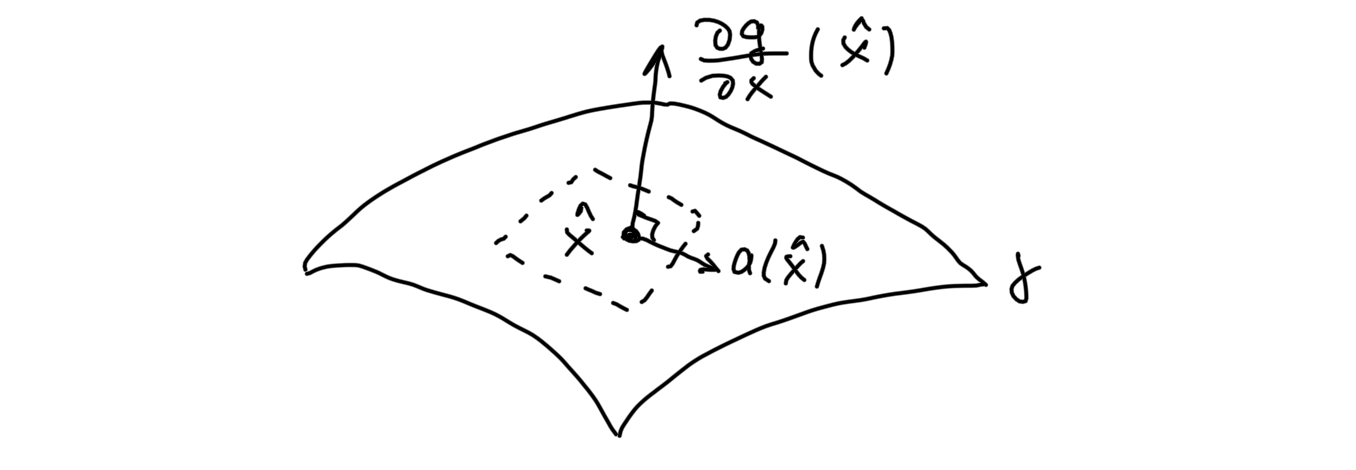
\includegraphics[scale=0.4]{characteristic-point}
    \centering
    \caption{Визуализация характеристической точки}
\end{figure}

\textbf{Теорема.} Пусть точка $\widehat{x} \in \gamma$ не является характеристической.
Тогда существуют окрестность $V(\widehat x)$ и функция $u\colon V(\widehat{x}) \to \mathbb R$ такая, что она является единственным решением задачи (3) в этой окрестности.

\textbf{Доказательство.} Мы знаем, что $a(\widehat{x}) \ne 0$. Тогда можно применить одно из предложений выше: существуют окрестность $X(\widehat{x})$ и функции $u_2, \dots, u_n \colon X(\widehat{x}) \to \mathbb{R}$ такие, что 
$u_2, \dots, u_n$ -- функционально независимые решения задачи (1). 

Зададим отображение $\Phi\colon X(\widehat{x}) \to \mathbb{R}^n$ следующим образом:
$$
\Phi(x) \coloneq 
\begin{pmatrix}
    g(x)\\
     u_2(x)\\
     \vdots\\
     u_n(x)\\
\end{pmatrix}.
$$
Хотим применить теорему об обратной функции, проверим, что матрица Якоби
\[ 
    \begin{pmatrix}
        \frac{\partial g}{\partial x}(\widehat{x}) \\[5pt]
        \frac{\partial u_{2}}{\partial x}(\widehat{x}) \\
        \vdots \\
        \frac{\partial u_{n}}{\partial x}(\widehat{x})
    \end{pmatrix}
\]
невырождена. Докажем от противного: пусть
\[
    \frac{\partial g}{\partial x}(\widehat x) = \sum_{j=2}^{n} \lambda_j \frac{\partial u_j}{\partial x}(\widehat x).
\]
Это рассматривать достаточно, так как первые $n - 1$ строк точно линейно независимы.
Умножим скалярно на $a(\widehat x)$:
\[
    \left< a(\widehat x), \frac{\partial g}{\partial x}(\widehat x) \right> = \sum_{j=2}^{n} \lambda_j \left< a(\widehat x), \frac{\partial u_j}{\partial x}(\widehat x) \right> = 0,
\]
так как $u_j$ --- решения уравнения (1).
Противоречие с тем, что $\widehat x$ не является характеристической точкой. 

Теперь по теореме об обратном отображении найдутся окрестности $V(\widehat x) \subset X(\widehat{x})$,\\
$W((u_2(\widehat x), \dots, u_{n}(\widehat x))) \subset \mathbb{R}^{n-1}$ и $\varepsilon > 0$ такие, что $\Phi \colon V \to (-\varepsilon, \varepsilon) \times W$ является диффеоморфизмом. Построим решение задачи Коши. Возьмём функцию $$u(x) \coloneq \phi(\Phi^{-1}(0, u_2(x), \dots, u_n(x)))$$
для всех $x \in V(\widehat{x})$. Заметим, что $u$ -- решение уравнения (1). Покажем, что $u$ также является решением задачи Коши. Берём $x \in \gamma \Rightarrow g(x) = 0$:
$$u(x) = \phi(\Phi^{-1}(0, u_2(x), \dots, u_n(x))) = \phi(\Phi^{-1}(g(x), u_2(x), \dots, u_n(x))) = \phi(\Phi^{-1}(\Phi(x))) = \phi(x).$$
Таким образом, мы доказали существование решения. Докажем теперь единственность.

Для этого уменьшим окрестности $V$, $W$ и $\varepsilon$ так, чтобы для любого решения $v \colon V \to \mathbb{R}$ уравнения (1) существовала функция $F \in C^1(W, \mathbb{R}) : v(x) \equiv F(u_2(x), \dots, u_n(x))$.
Возьмём на меньшей окрестности решение $v \colon V \to \mathbb{R}$ задачи Коши (3) и покажем, что оно совпадает с уже найденным решением $u$.

Во-первых, для него выполняется $v(x) \equiv F(u_2(x), \dots u_n(x))$. Возьмём $x \in \gamma \Rightarrow v(x) = \phi(x) = u(x)$, так как и $u, v$ являются решениями задачи Коши. Значит, $F(u_2(x), \dots u_n(x)) \equiv \phi(\Phi^{-1}(0, u_2(x), \dots, u_n(x)))$.
Поскольку $\Phi$ --- это диффеоморфизм, то для любой точки\\$(y_1, \dots, y_n) \in W$ верно: $F(y_2, \dots, y_n) \equiv \phi(\Phi^{-1}(0, y_2, \dots, y_n)).$
Тогда $$v(x) \equiv F(u_2(x), \dots, u_n(x)) \equiv \phi(\Phi^{-1}(0, u_2(x), \dots, u_n(x))) \equiv u(x).$$

\QED

\textbf{Пример.} Рассмотрим уравнение $u_x + u_y = 0$ и начальное условие
$$
\begin{cases}
  u(x, y) = 1\\
  x-y = 0
\end{cases}.
$$
Перейдем к характеристической системе 
$$
 \begin{cases}
    x' = 1\\
    y' = 1
 \end{cases}.
$$
Тогда $x - y = C$ --- это первый интеграл. Рассмотрим произвольную функцию $F$: $F(0) = 1$.
Отсюда $u(x, y) = F(x-y)$ является решением задачи Коши, то есть решений бесконечно много.

Рассмотрим теперь то же уравнение, но с другим начальным условием:
$$
\begin{cases}
   u(x, y) = x^2+y^2\\
   x-y = 0
\end{cases}.
$$

Знаем, что $u(x, y) = F(x-y)$ --- это общее решение. При $x-y = 0$ получаем $u(x, y) = F(0)$. Значит, для всех решений задачи Коши $F(0) = x^2+y^2$ на прямой $x-y = 0$. Такого быть не может, потому что $F(0)$ --- константа. То есть у этой задачи Коши нет решений. 

В этих примерах не выполняется условие теоремы, потому что все точки на кривой $\gamma$ являются характеристическими.

Действительно,
$$
a =
\begin{pmatrix}
1\\
1
\end{pmatrix},\;\;
\frac{\partial g}{\partial x} =
\begin{pmatrix}
1\\
-1
\end{pmatrix},
$$
а их скалярное произведение равно нулю во всех точках.
% \section{Оффтоп: ОДУ и случайные графы}
% Ответ на вопрос, зачем нам дифференциальные уравнения, если у нас нет физики.
% На экзамене не будет.

% Везде неявно фиксируется индекс $n$.
% Пусть $(\Omega, \mathcal F, P)$ --- вероятностное пространство, $\mathcal F_0 \subset \mathcal F_1 \subset \dots \subset \mathcal F$, где $\mathcal F_0 = \{\varnothing, \Omega\}$, а $\mathcal F_t = \sigma(A_1^t, \dots, A_{m(t)}^t)$, и $\Omega = \bigsqcup_{l=1}^{m(t)} A_l^t$ для всех $t$.
% Неформально мы берём множество $\Omega$ и постепенно разбиваем его на более мелкие куски.
% Пусть $a = a(n) \in \mathbb N$, $(Y_1(t), \dots, Y_a(t))$ --- случайные $\mathcal F_t$-измеримые величины.
% Предположим, что существует $c_0$, такое что для всех $i$ $|Y_i(t)| \le c_0 n$.

% \textbf{Теорема 1.} Пусть $D \subset \mathbb R^{a+1}$ --- открытое, связное и ограниченное множество, такое что $(0, Y_1(0)/n, \dots, Y_a(0)/n) \in D$.
% Положим 
% \[
%     T_D = \min \left\{ t \in \mathbb N \cup \{+\infty\}: \left( \frac{t}{n}, \frac{Y_1(t)}{n}, \dots, \frac{Y_a(t)}{n} \right) \not\in D \right\}
% \]
% --- случайная величина.
% Пусть даны функции $f_i: \mathbb R^{a+1} \to \mathbb R$, $f_i \in C^1$, $1 \le i \le a$.
% Зафиксируем $\beta > 0$ (не зависит от $n$), $\lambda = \lambda(n) = \mathcal O(1)$.
% Предположим, что для любого $t$ и $\omega \in \{t < T_D\}$ величина $\max |Y_i(t+1) - Y_i(t)| \le \beta$, а также для любого $t$, $i = \overline {1, a}$ и $A_l^t \subset \{t < T_D\}$ верно
% \[
%     \left| E(Y_i(t + 1) - Y_i(t)~|~A_l^t) - f_i \left(\frac{t}{n}, \frac{Y_1(t)}{n}, \dots, \frac{Y_a(t)}{n} \right) \right| \le \lambda.
% \]
% Тогда:
% \begin{itemize}
%     \item Задача Коши
%         \[
%             \begin{cases}
%                 z_i' = f_i(x, z_1, \dots, z_a) \\
%                 z_i(0) = \frac{1}{n} Y_i(0)
%             \end{cases}
%         \]
%         имеет единственное решение, продолжаемое до $\partial D$.
%         Далее зафиксируем это решение $z_i$.

%     \item Существует число $C > 0$, такое что для любых $i$ и $t \le \sigma \cdot n$
%         \[
%             Y_i(t) = n \cdot z_i \left( \frac{t}{n} \right) + \mathcal O(\lambda n)
%         \]
%         с вероятностью $1 - \mathcal O \left(\frac{e^{-\frac{n \lambda^3}{\beta^3}}}{\lambda} \right)$, где $\sigma$ --- такое число, что $\rho_{\infty}((x, z(z)), \partial D) \ge C\lambda$ для любого $x \in [0, \sigma]$.
% \end{itemize}

% \subsection{Процесс минимальных степеней}
% Рассмотрим последовательность графов $G_0, G_1, \dots, G_{C_n^2}$, где каждый следующий граф получен следующим образом: берём равновероятно вершину наименьшей степени, равновероятно выбираем другую вершину, в которую нет ребра, и проводим ребро ($G_0$ --- пустой граф).
% Обозначим $\Delta(G)$ --- наименьшая степень вершины в $G$ и $Y_i(t)$ --- количество вершин степени $i$ в графе $G_t$.
% Положим $f_i(x, z_0, z_1, \dots, z_{n-1}) = -I\{i = 0\} + I\{I = 1\} + z_{i-1} - z_i$.
% Рассмотрим задачу Коши
% \[
%     \begin{cases}
%         z_i = -I\{i = 0\} + I\{i = 1\} + z_{i-1} - z_i \\
%         z_0(0) = \frac{1}{n} Y_0(0) = 1 \\
%         z_i(0) = \frac{1}{n} Y_i(0) = 0
%     \end{cases}
% \]
% (здесь $z_{-1} \equiv 0$)
% Решая это уравнение по индукции, получаем решение
% \[
%     \begin{cases}
%         z_0(x) = 2e^{-x} - 1 \\
%         z_i(x) = 2 \frac{x^i}{i! e^x}
%     \end{cases}.
% \]

% \textbf{Теорема 2.} 
% \[
%     Y_i(t) = nz_i \left( \frac{t}{n} \right) + \mathcal O(n^{3/4})
% \]
% с вероятностью $1 - n^{3/4} \cdot e^{-\frac{n^{1/4}}{8}}$ для любого $n$ достаточно большого, $i < n$ и $t \le n \ln(2) - n^{4/5}$.

% \textbf{Доказательство.} Будем подгонять под теорему 1.
% Пусть $\Omega$ --- последовательности таких графов, которые мы строим.
% Положим 
% \[
%     \mathcal F_1 = \sigma \{\{\omega: G_0 = \widehat G_0\}~|~\widehat G_0\}.
% \]
% Теперь 
% \[
%     \mathcal F_2 = \sigma \{\{\omega: G_0 = \widehat G_0, G_1 = \widehat G_1 \}~|~\widehat G_0, \widehat G_1\}.
% \]
% И так далее.
% Положим для всех $t$ множество $S_t = \{\Delta(G_t) = 0\} \subset \Omega$ и случайную величину $X_i(t)$ --- индикатор того, что степень вершины, в которую проведено новое ребро, равно $i$.
% Тогда для $\omega S_t$ верно, что $X_0(t) \omega = 1$ тогда и только тогда, когда новое ребро проведено между вершинами степени 0, а $X_i(t) \omega = 1$ тогда и только тогда, когда мы провели ребро в вершину степени $i$.
% Заметим, что для $\omega \in S_t$
% \[
%     Y_0(t + 1) = Y_0(t) - 1 - X_0(t).
% \]
% Аналогично можно написать для всех:
% \[
%     Y_1(t + 1) = Y_1(t) + 1 + X_0(t) - X_1(t),
% \]
% \[
%     Y_{i+1}(t) = Y_i(t) + X_{i-1}(t) - X_i(t).
% \]
% Найдём математическое ожидание:
% \[
%     E(Y_0(t + 1) - Y_0(t)~|~\{G_t = \widehat G_t\}) = -1 - \frac{Y_0(t) - 1}{n - 1}.
% \]
% Справа случайная величина, потому что слева --- тоже, математическое ожидание зависит от $\omega = (\dots, \widehat G_t, \dots)$.
% Аналогично
% \[
%     E(Y_1(t + 1) - Y_1(t)~|~\{G_t = \widehat G_t\}) = 1 + \frac{Y_0(t) - 1}{n - 1} - \frac{Y_1(t)}{n - 1}
% \]
% и
% \[
%     E(Y_i(t + 1) - Y_i(t)~|~\{G_t = \widehat G_t\}) = \frac{Y_{i-1}(t) - 1}{n - 1} - \frac{Y_i(t)}{n - 1}.
% \]
% Положим
% \[
%     D - \left\{(x, z) \in \mathbb R^{n+1}: -1 < x < \frac{n}{2}, z_0 > 0, -1 < z_i < 2\right\}.
% \]
% Здесь важно, что все $z_i \in (-1, 2)$, но $z_0 \in (0, 2)$.
% Теперь возьмём $a = n$, $c_0 = 1$ и проверим, что предположение теоремы выполняется.
% Для вектора $\left( \frac{t}{n}, \frac{Y_0(t)}{n}, \dots, \frac{Y_{n-1}(t)}{n} \right)$ выполняется, что $0 \le \frac{Y_i(t)}{n} \le 1$ и $\frac{t}{n} \ge 0$.
% Тогда событие $t < T_D$ --- это ``существует вершина степени ноль в графах $G_0, \dots, G_t$``, то есть $S_t$.
% Нужно ограничение на разность $|Y_i(t + 1) - Y_i(t)|$.
% Его получить нетрудно, ибо при проведении ребра количество вершин степени $i$ изменилось не более, чем на 2 --- положим $\beta := 2$.
% Оценим разность
% \[
%     \left| E(Y_i(t + 1) - Y_i(t)~|~\{G_t = \widehat G_t\}) - f_i \left( \frac{t}{n}, \frac{Y_0(t)}{n}, \dots, \frac{Y_{n-1}(t)}{n} \right) \right| = 
% \]
% \[
%     = \left| \frac{Y_{i-1}(t) - Y_i(t)}{n - 1} - \frac{Y_{i-1}(t) - Y_i(t)}{n} \right| = \frac{|Y_{i-1}(t) - Y_i(t)|}{n(n-1)} \le
% \]
% \[
%     \le \frac{|Y_{i-1}(t)| + |Y_i(t)|}{n(n - 1)} \le \frac{1}{n-1} \le n^{-1/4} =: \lambda.
% \]
% Все условия выполнены, поэтому по второму следствию теоремы получаем, что найдётся $c > 0$, такое что и так далее.
% Заметим, что $z_i(x) \in [0, 1]$ при $x \ge 0$, а $z_0(x) \in (0, 1]$ при $x \in [0, \ln(2))$ и $z_0(\ln(2)) = 0$.
% Засчёт гениального подгона условий во множестве $D$, мы получаем, что $\dist_\infty((x, z(x)), \partial F) = z_0(x)$, так как по остальным координатам есть большой запас.
% В то же время $z_0(\ln(2) - n^{-1/5}) \approx n^{-1/5} >> cn^{-1/4} = c\lambda$.
% Теперь берём $\sigma = \ln(2) - n^{-1/5}$ и получаем что-то интересное.

% \QED

% \setcounter{equation}{0}
% \section{Оффтоп: производящие функции}
% \subsection{Линейные рекуррентные соотношения}
% Рассмотрим рекуррентное соотношение
% \begin{equation}
%     a_0 u_{n+k} + a_1 u_{n+k-1} + \dots + a_n u_k = 0.
% \end{equation}
% Её решением является какая-то последовательность $\{u_k\}_{k=0}^\infty$.
% Также будем считать, что нам известны первые $n - 1$ членов $\widehat u_0, \dots, \widehat u_{n-1}$ --- очень похоже на задачу Коши.
% Рассмотрим экспоненциальную производящую функцию
% \[
%     x(t) = \sum_{j=0}^{\infty} \frac{u_j t^j}{j!}.
% \]
% Её производная ---
% \[
%     x'(t) = \sum_{j=0}^{\infty} \frac{u_{j+1} t^j}{j!}.
% \]
% В общем случае
% \[
%     x^{(n)}(t) = \sum_{j=0}^{\infty} \frac{u_{j+n} t^j}{j!}.
% \]
% Рассмотрим линейную комбинацию $a_0 x^{(n)} + \dots + a_{n-1} x' + a_n x$.
% Она равна
% \[
%     \sum_{j=0}^{\infty} \frac{t^j}{j!} (a_0 u_{j+n} + \dots + a_{n-1} u_{j+1} + a_n u_j).
% \]

% \textbf{Теорема.} Пусть $x(\cdot)$ --- это решение задачи Коши
% \[
%     \begin{cases}
%         a_0 x^{(n)} + \dots + a_{n-1} x' + a_n x = 0 \\
%         x(0) = \widehat u_0, \dots, x^{(n-1)}(0) = \widehat u_{n-1}
%     \end{cases}.
% \]
% Тогда $\{u_k\}$ является решением (1), они берутся из разложения $x(t)$ в ряд.

% \subsection{Числа Стирлинга второго рода}
% \textbf{Определение.} Пусть $n \ge k$. \textit{Числом Стирлинга второго рода} $S(n, k)$ называется количество неупорядоченных разбиений $n$-элементного множества на $k$ неупорядоченных подмножеств.

% В частности, $S(n, 0) = 0$ при $n > 0$, $S(0, 0) = 1$ и $S(n, k) = S(n - 1, k - 1) + k \cdot S(n - 1, k)$.
% Более того,
% \[
%     S(n, k) = \frac{1}{k!} \sum_{j=0}^{k} (-1)^{k+1} C_k^j \cdot j^n.
% \]
% Рассмотрим экспоненциальный степенной ряд
% \[
%     x_k(t) = \sum_{n=k}^{\infty} S(n, k) \frac{t^n}{n!}.
% \]
% Используя рекурренту, получаем
% \[
%     x_k(t) = \sum_{n=k}^{\infty} (S(n - 1, k - 1) + k \cdot S(n - 1, k)) \cdot \frac{t^n}{n!}.
% \]
% Формально продифференцируем:
% \[
%     x'_k(t) = \sum_{n=k}^{\infty} S(n - 1, k - 1) \cdot \frac{t^{n-1}}{(n-1)!} + k \cdot \sum_{n=k}^{\infty} S(n - 1, k) \cdot \frac{t^{n-1}}{(n-1)!}.
% \]
% Во второй сумме получилась неприятность в виде того, что нам нужно $S(n - 1, n)$, а мы такое не определяли, поэтому доопределим нулём.
% Методом пристального взгляда заключаем, что $x'_k(t) = x_{k-1}(t) + k \cdot x_k(t)$.
% Остаётся найти $x_0(t) = \sum_{n = 0}^{\infty} S(n, 0) \cdot \frac{t^n}{n!} = 1$, и мы научились находить $x_k$ решением задачи Коши с добавлением условия $x_k(0) = 0$.
% Можно проверить, что $x_k(t) = \frac{1}{k!} (e^t - 1)^k$.

% \setcounter{equation}{0}
% \section{Линейные однородные уравнения в частных производных}
% Пусть $\Omega \subset \mathbb R^n$ --- область, $a: \Omega \to \mathbb R^n$ --- вектор-функция, $a \in C^1$.
% Рассмотрим уравнение
% \begin{equation}
%     a_1(x) \cdot \frac{\partial u}{\partial x_1}(x) + \dots + a_n(x) \cdot \frac{\partial u}{\partial x_n}(x) = 0.
% \end{equation}
% Его решением является функция $u: D \to \mathbb R$, где $D \subset \Omega$ --- область и $u \in C^1$, при подстановке которой получается тождественный ноль.
% В сокращённой записи
% \[
%     \left< a(x), \frac{\partial u}{\partial x}(x) \right> = 0.
% \]

% \textbf{Определение.} Такое уравнение называется \textit{линейным однородным уравнением в частных производных первого порядка}.

% \textbf{Определение.} Система
% \begin{equation}
%     x' = a(x)
% \end{equation}
% называется \textit{характеристической системой} уравнения.

% Найдём связь между решениями уравнения (1) и его характеристической системы (2).
% Пусть $\overline x \in \Omega$ --- какая-то точка, причём $a(\overline x) \ne 0$.

% \textbf{Теорема.} 1) Любой первый интеграл системы (2) является решением системы (1).

% 2) Пусть $v_1, \dots, v_{n-1}: \Omega \to \mathbb R$ --- независимые первые интегралы системы (2).
% Тогда существует окрестность $D$ точки $\overline x$, такая что для любого решения $u: D \to \mathbb R$ уравнения (1) существует гладкая функция $F$, такая что $u(x) \equiv F(v_1(x), \dots, v_{n-1}(x))$.

% \textbf{Доказательство.} 1) Пусть $u(\cdot)$ --- первый интеграл (2).
% По критерию первого интеграла $\left<a(x), \frac{\partial u}{\partial x}(x) \right> \equiv 0$, что мы и хотели.

% 2) По теореме о первом интеграле существует окрестность $D$, такая что любой первый интеграл в ней представим в виде $F(v_1(x), \dots, v_{n-1}(x))$.
% Рассмотрим произвольное решение $u: D \to \mathbb R$ уравнения (1).
% Раз решение, то $\left<a(x), \frac{\partial u}{\partial x}(x) \right> \equiv 0$, а значит, $u(\cdot)$ --- первый интеграл системы (2), то есть имеет искомое представление в окрестности $D$.

% \QED

% Пусть заданы гладкие функции $g, \phi: \Omega \to \mathbb R$, причём $\frac{\partial g}{\partial x}(x) \ne 0$ на $\Omega$, и $g(\overline x) = 0$.
% Тогда существует непустое множество $\gamma := \{x: g(x) = 0\}$, более того, это $(n-1)$--мерная поверхность.
% Рассмотрим задачу Коши
% \begin{equation}
%     \begin{cases}
%         \left<a(x), \frac{\partial u}{\partial x}(x) \right> \equiv 0 \\
%         u(x) = \phi(x) \text{ при $x \in \gamma$}
%     \end{cases}.
% \end{equation}
% Как и у любой уважающей себя задачи Коши, для неё есть теорема о существовании и единственности решения, но это чуть позже.

% \textbf{Определение.} $\overline x$ называется \textit{характеристической точкой} задачи (3), если $\left<a(\overline x), \frac{\partial u}{\partial x}(\overline x) \right> = 0$.

% \textbf{Теорема.} Пусть точка $\overline x$ не является характеристической.
% Тогда существует окрестность $D$ точки $\overline x$ и функция $u: D \to \mathbb R$, такая что $u$ является единственным решением (3) в этой окрестности.

% \textbf{Доказательство.} Мы знаем, что $a(\overline x) \ne 0$.
% Поэтому можно применить теорему о первых интегралах: существует область $\widetilde D$ точки $\overline x$, в которой есть независимые первые интегралы $v_1, \dots, v_{n-1}: \widetilde D \to \mathbb R$ системы (2).
% Рассмотрим систему
% \[
%     \begin{cases}
%         v_1(x) = u_1 \\
%         \vdots \\
%         v_{n-1}(x) = u_{n-1} \\
%         g(x) = \Theta
%     \end{cases}.
% \]
% (здесь все значения в правых частях --- это параметры)
% Хотим применить теорему об обратной функции, проверим, что условия выполнены.
% Для этого рассмотрим матрицу Якоби:
% \[
%     A = 
%     \begin{pmatrix}
%         \frac{\partial v_1}{\partial x}(\overline x) \\
%         \vdots \\
%         \frac{\partial v_{n-1}}{\partial x}(\overline x) \\
%         \frac{\partial g}{\partial x}(\overline x) \\
%     \end{pmatrix}
% \]
% Докажем от противного, что она невырождена: пусть
% \[
%     \frac{\partial g}{\partial x}(\overline x) = \sum_{j=1}^{n-1} \lambda_j \frac{\partial v_j}{\partial x}(\overline x).
% \]
% Это рассматривать достаточно, так как первые $n - 1$ строк точно линейно независимы.
% Тогда
% \[
%     \left< a(\overline x), \frac{\partial g}{\partial x}(\overline x) \right> = \sum_{j=1}^{n-1} \lambda_j \left< a(\overline x), \frac{\partial v_j}{\partial x}(\overline x) \right> = 0,
% \]
% так как это первые интегралы.
% Противоречие с тем, что $\overline x$ не является характеристической точкой.

% Теперь по теореме об обратной функции найдётся окрестность $\Gamma$ точки $(v_1(\overline x), \dots, v_{n-1}(\overline x), 0)$ (в конце ноль, так как $g(\overline x) = 0$) и $\chi: \Gamma \to \mathbb R^n$, $\chi \in C^1$, такие что
% \[
%     \begin{cases}
%         v_1(\chi(u_1, \dots, u_{n-1}, \Theta)) = u_1 \\
%         \vdots \\
%         v_{n-1}(\chi(u_1, \dots, u_{n-1}, \Theta)) = u_{n-1} \\
%         g(\chi(u_1, \dots, u_{n-1}, \Theta)) = \Theta \\
%     \end{cases}
% \]
% и
% \[
%     \chi(v_1(x), \dots, v_{n-1}(x), g(x)) \equiv x.
% \]
% Тогда $\chi(u_1, \dots, u_{n-1}, \Theta)$ является единственным решением построенной системы, причём $\chi(v_1(\overline x), \dots, v_{n-1}(\overline x), 0) = \overline x$.

% Теперь восстановим единственное решение задачи Коши.
% Положим $u(x) := \phi(\chi(v_1(x), \dots, v_{n-1}(x), 0))$.
% Возьмём достаточно малую окрестность $D$ точки $\overline x$, такую что для всех $x \in D$ выполнено $(v_1(x), \dots, v_{n-1}(x), 0) \in \Gamma$.

% Почему это решение уравнения в частных производных? Потому что взяли гладкую функцию от первых интегралов.
% \sloppy Почему это решение задачи Коши? При $x \in \gamma$ выполнено $g(x) = 0$, то есть $u(x) = \phi(\chi(v_1(x), \dots, v_{n-1}(x), g(x))) = \phi(x)$, так как обратная функция.

% Единственность остаётся в качестве упражнения.
% Доказательство от автора конспекта: рассмотрим произвольное решение $F(v_1, \dots, v_{n-1})$ и точку $x_1 \in D$.
% Положим $x_2 = \chi(v_1(x_1), \dots, v_{n-1}(x_1), 0) \in \gamma$.
% Заметим, что $v_i(x_2) = v_i(x_1)$ для всех $i$, так как $\chi$ --- обратная к отображению $x \mapsto (v_1(x), \dots, v_{n-1}(x), g(x))$.
% Следовательно, $F(v_1(x_1), \dots, v_{n-1}(x_1)) = F(v_2(x_2), \dots, v_{n-1}(x_2)) = \phi(x_2)$, то есть $F(v_1, \dots, v_{n-1})$ однозначно определено в $x_1$.

% \QED

\section{Вариационное исчисление}
\subsection{Простейшая задача вариационного исчисления}
Рассмотрим пространство функций $C^1[a, b]$, как нормированное пространство, и его подмножество $M$.
Зададим на нём метрику $\rho(x_1, x_2) = \max_{t \in [a, b]} |x_1(t) - x_2(t)|$ и $\rho_1(x_1, x_2) = \rho(x_1, x_2) + \rho(x_1', x_2')$.
Пусть у нас есть функционал $I: M \to\ \mathbb R$.

\textbf{Определение.} Точка $\widehat x \in M$ называется \textit{слабым локальным минимумом} функционала $I$, если $\exists \varepsilon > 0: \forall x \in M~(\rho_1(x, \widehat x) < \varepsilon \Rightarrow I(\widehat x) \le I(x))$
Аналогично для максимума.

\textbf{Определение.} Точка $\widehat x \in M$ называется \textit{сильным локальным минимумом}, если вместо $\rho_1$ используется $\rho$.

\textbf{Утверждение.} Если $\widehat x$ --- сильный локальный минимум, то он также является слабым. Очевидно.

Рассмотрим дважды гладко дифференцируемую (в $C^2$) функцию $F: \mathbb R^3 \to \mathbb R$ и числа $A, B \in \mathbb R$.
Положим
\[
    M = \{x \in C^1[a, b]: x(a) = A, x(b) = B\}
\]
и
\[
    I(x) := \int_a^b F(t, x(t), x'(t)) dt, x \in M.
\]

\textbf{Определение.} \textit{Простейшей задачей вариационного исчисления} называется задача нахождения слабых локальных экстремумов функционала $I$.

Положим
\[
    \mathring C^1[a, b] := \{x \in C^1[a, b]: x(a) = x(b) = 0\}.
\]
Тогда множество $M$ замкнуто относительно прибавления функций из $\mathring C^1[a, b]$.

Положим для $\widehat x \in M$, $\widehat x \in C^2$, $\eta \in \mathring C^1[a, b]$ функцию
\[
    \phi(\mu) := I(\widehat x + \mu \eta) = \int_a^b F(t, \widehat x(t) + \mu \eta(t), \widehat x'(t) + \mu \eta'(t)) dt.
\]
Продифференцируем её:
\[
    \phi'(\mu)|_{\mu = 0} = \int_a^b \left( \frac{\partial F}{\partial x}(t, \widehat x(t), \widehat x'(t)) \eta(t) + \frac{\partial F}{\partial x'}(t, \widehat x(t), \widehat x'(t)) \eta'(t) \right) dt =
\]
Проинтегрируем по частям:
\[
    = \int_a^b \frac{\partial F}{\partial x}(t, \widehat x(t), \widehat x'(t)) \eta(t) dt + \frac{\partial F}{\partial x'}(\dots) \eta(t) \big|_a^b - \int_a^b \frac{d}{dt} \frac{\partial F}{\partial x'}(\dots) \eta(t) dt =
\]
Второе слагаемое рано нулю, так как $\eta(a) = \eta(b) = 0$
\[
    = \int_a^b \left(\frac{\partial F}{\partial x}(\dots) - \frac{d}{dt} \frac{\partial F}{\partial x'}(\dots) \right) \eta(t) dt.
\]
Таким образом, если $\widehat x$ является слабым локальным минимумом, то 0 --- стационарная точка функции $\phi$.

\textbf{Определение.} $\delta I[\widehat x, \eta] := \phi'(0)$ --- первая вариация функционала $I$ на $\widehat x$.

\textbf{Утверждение.} Если $\widehat x \in M$ --- слабый локальный экстремум, то для любого $\eta \in \mathring C^1[a, b]$ точка $0$ является локальным экстремумом функции $\phi$.

\textbf{Доказательство.} Будем считать, что мы работаем с точкой минимума.
По определению существует $\varepsilon > 0$, такое что для любого $x \in M$, удовлетворяющему $\rho_1(x, \widehat x) < \varepsilon$ верно $I(x) \ge I(\widehat x)$.

Тогда для любого $\eta \in \mathring C^1[a, b]$, не равного тождественному нулю, положим $\delta = \frac{\varepsilon}{\rho_1(\eta, 0)}$.
Возьмём произвольный $\mu \in (-\delta, \delta)$.
Имеем
\[
    \rho_1(\widehat x + \mu \eta, \widehat x) = \max_{t \in [a, b]} |\mu \eta(t)| + \max_{t \in [a, b]} |\mu \eta'(t)| =
\]
\[
    = |\mu| \left( \max_{t \in [a, b]} |\eta(t)| + \max_{t \in [a, b]} |\eta'(t)| \right) = |\mu| \cdot \rho_1(\eta, 0) < \varepsilon.
\]
Таким образом, мы попали в $\varepsilon$-окрестность функции $\widehat x$, то есть $\phi(\mu) = I(\widehat x + \mu \eta) \ge I(\widehat x) = \phi(0)$.

\QED

\textbf{Утверждение.} (Лемма Лагранжа) Пусть $v \in C[a, b]$, такая что $\forall \eta \in \mathring C^1[a, b]$ выполнено
\[
     \int_a^b v(t) \eta(t) dt = 0.
\]
Тогда $v(t) \equiv 0$.

\textbf{Доказательство.} От противного: допустим, что существует $\tilde \tau \in [a, b]$, такое что $v(\tilde \tau) > 0$.
Тогда существует $\tau \in (a, b)$, такое что $v(\tau) > 0$ из непрерывности.
Отсюда существует $\varepsilon > 0$, такой что $(\tau - \varepsilon, \tau + \varepsilon) \subset [a, b]$ и $v(t) > \frac{v(\tau)}{2}$ для $t \in (\tau - \varepsilon, \tau + \varepsilon)$.

Теперь построим гладкую функцию, принимающую положительные значения на $T := (\tau - \varepsilon, \tau + \varepsilon)$ и ноль вне этого интервала.
В частности,
\[
    \eta(t) :=
    \begin{cases}
        (t - (\tau - \varepsilon))^2 (t - (\tau + \varepsilon))^2, & t \in T \\
        0, & \text{иначе}
    \end{cases}.
\]
Отсюда по условию
\[
    0 = \int_a^b v(t) \eta(t) dt = \int_T v(t) \eta(t) dt.
\]
Противоречие, так как мы взяли интеграл по непустому интервалу произведения двух положительных функций.

\QED

\textbf{Теорема.} Пусть $F \in C^2$, $\widehat x \in M$, $\widehat x \in C^2$ --- слабый локальный экстремум.
Тогда $\widehat x$ является решением уравнения Эйлера
\[
    \frac{\partial F}{\partial x} (t, x, x') - \frac{d}{dt} \frac{\partial F}{\partial x'} (t, x, x') = 0.
\]

\textbf{Доказательство.} Поскольку $\widehat x$ является слабым локальным экстремумом, по утверждению для любой $\eta \in \mathring C^1[a, b]$ точка $0$ является локальным экстремумом функции $\phi$, то есть $\phi'(0) = 0$.
Выражение для $\phi'(0)$ мы уже писали выше --- теперь заметим, что по утверждению про локальный экстремум $\phi$ получаем $\phi'(0) = 0$, а по лемме Лагранжа ---
\[
    \frac{\partial F}{\partial x} (t, \widehat x, \widehat x'(t)) - \frac{d}{dt} \frac{\partial F}{\partial x'} (t, \widehat x, \widehat x'(t)) \equiv 0.
\]
Следовательно, $\widehat x$ является решением уравнения Эйлера.

\QED

\textbf{Замечание.} Повсюду мы говорили, что $\widehat x \in C^2$.
Но теоретически экстремумом может являться и функция из $C^1$.
Пусть $F, \widehat x \in C^1$.
Если $\widehat x$ --- слабый локальный экстремум, то функция
\[
    t \mapsto \frac{\partial F}{\partial x'} (t, \widehat x(t), \widehat x'(t))
\]
непрерывно дифференцируема, и $\widehat x$ является решением уравнения Эйлера.
Иными словами, прошлая теорема верна и в этом случае, но доказывать мы это не будем.

\textbf{Определение.} Решение уравнения Эйлера называется \textit{экстремальным}.
Тогда прошлую теорему можно переформулировать, как ``слабый локальный экстремум является экстремальным``.

\subsection{Задача о брахистохроне}
Людям с острой непереносимостью физики рекомендуется пропустить.
Остальным: для понимания достаточно школьных знаний.

Пусть у нас есть две материальные точки $A$ и $B$, причём $A$ выше $B$.
Мы хотим провести между ними кривую, такую что материальная точка, двигаясь по ней исключительно под силой тяжести, достигнет точку $B$ за минимальное время.
Эта кривая называется \textit{брахистрохоной}.

% \begin{figure}[ht]
%     \centering
%     \incfig{811}{0.5\linewidth}
% \end{figure}

Запишем закон сохранения энергии:
\[
    mg \cdot y(x) = \frac{m v^2(x)}{2}.
\]
Тогда
\[
    v(x) = \sqrt {2g \cdot y(x)}.
\]
Запишем скорость, как производную от пройденного пути $s$:
\[
    v(x) = \frac{ds}{dt} = \frac{ds}{dx} \cdot \frac{dx}{dt} = \frac{d}{dx} \int_0^x \sqrt{ 1 + (y'(\xi))^2 } d\xi \cdot \frac{dx}{dt} = \sqrt{1 + (y'(x))^2} \cdot \frac{dx}{dt}.
\]
Выразим $dt$:
\[
    dt = \frac{\sqrt{1 + (y'(x))^2}}{\sqrt{2g \cdot y(x)}} dx,
\]
то есть
\[
    t = \int_0^b \sqrt{ \frac{1 + (y'(x))^2}{2g \cdot y(x)}} \cdot dx.
\]
Итак, итак, простейшая вариационная задача.
Выкинем лишние константы:
\[
    t(y) = \int_0^b \sqrt{ \frac{1 + (y')^2}{y}} dx \to \min.
\]
Здесь $y(0) = 0$, $y(b) = B$.
Уравнением Эйлера будем
\[
    \sqrt{1 + (y')^2} \left( -\frac{1}{2} \cdot \frac{1}{(\sqrt y)^3} \right) - \frac{d}{dx} \cdot \frac{2y'}{\sqrt y \cdot 2 \cdot \sqrt{1 + (y')^2}} = 0.
\]
Заметим, что это то же самое, что
\[
    \frac{d}{dx} \left( \sqrt{\frac{1 + (y')^2}{y}} - \frac{(y')^2}{\sqrt{y (1 + (y')^2)}} \right) = 0.
\]
То есть $y(y + (y')^2) = c_1$ --- константа.
Сделаем замену: $y'(x(\tau)) = \ctg(\tau)$.
Тогда 
\[
    y(x(\tau)) = c_1 \sin^2(\tau) = \frac{1}{2} c_1 (1 - \cos(2\tau)).
\]
Теперь
\[
    dx = \frac{dy}{y'} = \frac{2c_1 \sin(\tau) \cos(\tau)}{\ctg(\tau)} d\tau = c_1(1 - \cos(2\tau)) d\tau.
\]
Значит,
\[
    x(\tau) = c_2 + \frac{c_1}{2} (2\tau - \sin(2\tau)).
\]
Теперь остаётся проверить, какие из них являются экстремумами, делается напрямую.

\setcounter{equation}{0}
\subsection{Задача со свободным концом}
Пусть $F: \mathbb R^3 \to \mathbb R \in C^2$, числа $a, b, A \in \mathbb R$ фиксированы.
Рассмотрим функционал
\begin{equation}
    I(x) = \int_a^b F(t, x(t), x'(t)) dt
\end{equation}
при условии $x(a) = A$.

Мы хотим найти экстремумы $I: M \to \mathbb R$, где $M = \{x \in C^1[a, b]: x(a) = A\}$.

\textbf{Теорема.} Пусть $\widehat x \in M$, $\widehat x \in C^2$ --- решение (1), то есть слабый локальный экстремум $I$.
Тогда $\widehat x$ является решением уравнения Эйлера
\[
    \frac{\partial F}{\partial x}(t, x, x') - \frac{d}{dt} \frac{\partial F}{\partial x'}(t, x, x') = 0,
\]
а также
\begin{equation}
    \frac{\partial F}{\partial x'}(b, \widehat x(b), \widehat x'(b)) = 0.
\end{equation}

\textbf{Доказательство.} Зафиксируем допустимое приращение $\eta \in C^1[a, b]$, $\eta(a) = 0$.
Положим
\[
    \Phi(\alpha) := I(\widehat x + \alpha \eta) = \int_a^b F(t, \widehat x(t) + \alpha \eta(t), \widehat x'(t) + \alpha \eta'(t)) dt.
\]
Найдём производную в нуле:
\[
    \Phi'(0) = \int_a^b \left( \frac{\partial F}{\partial x}(t, \widehat x(t), \widehat x'(t)) \eta(t) + \frac{\partial F}{\partial x'} (t, \widehat x(t), \widehat x'(t)) \eta'(t) \right) dt =
\]
Проинтегрируем по частям
\[
    = \int_a^b \frac{\partial F}{\partial x}(\dots)\eta(t) dt + \frac{\partial F}{\partial x'} (t, \widehat x(t), \widehat x'(t)) \eta(t) \bigg|_{t=a}^{t=b} - \int_a^b \frac{d}{dt} \frac{\partial F}{\partial x'}(\dots) \eta(t) dt =
\]
\[
    = \int_a^b \left( \frac{\partial F}{\partial x}(\dots) - \frac{d}{dt} \frac{\partial F}{\partial x'}(\dots) \right) \eta(t) dt + \frac{\partial F}{\partial x'}(b, \widehat x(b), \widehat x'(b)) \eta(b),
\]
так как $\eta(a) = 0$.

Как доказывалось в простейшей задаче вариационного исчисления, $0$ является локальным экстремумом функции $\Phi$, то есть $\Phi'(0) = 0$.
Таким образом, выражение выше равно нулю.

Подставим в выражение выше функцию $\eta$ с $\eta(b) = 0$, тогда останется только
\[
    \int_a^b \left( \frac{\partial F}{\partial x}(t, \widehat x(t), \widehat x'(t)) - \frac{d}{dt} \frac{\partial F}{\partial x'}(t, \widehat x(t), \widehat x'(t)) \right) \eta(t) dt = 0.
\]
По лемме Лагранжа получаем уравнение Эйлера.
Теперь остаётся только 
\[
    \frac{\partial F}{\partial x'} (b, \widehat x(b), \widehat x'(b)) \eta(b) = 0
\]
для всех функций $\eta$, то есть
\[
    \frac{\partial F}{\partial x'} (b, \widehat x(b), \widehat x'(b))  \equiv 0.
\]

\QED

\textbf{Замечание.} Опять же если $F, \widehat x \in C^1$, то функция
\[
    \frac{\partial F}{\partial x'}(t, \widehat x(t), \widehat x'(t))
\]
непрерывно дифференцируема по $t$, $\widehat x$ является решением уравнения Эйлера и выполняется (2).

\textbf{Замечание 2.} Можно рассматривать и задачу с другим свободным концом, тогда (2) будет иметь вид
\[
    \frac{\partial F}{\partial x'}(a, \widehat x(a), \widehat x'(a)) = 0.
\]
А если оба конца свободны, то условие выше и условие (2) выполняются одновременно.

\subsection{Задача для функционалов, зависящих от нескольких функций}
Пусть у нас есть функция $F: \mathbb R \times \mathbb R^n \times \mathbb R^n \to \mathbb R \in C^2$, заданы числа $a, b \in \mathbb R$ и $A, B \in \mathbb R^n$, где $A = (A_i)_{i = \overline{1, n}}$ и $B = (B_i)_{i = \overline{1, n}}$.

Рассмотрим задачу нахождения экстремумов функционала
\begin{equation}
    I(x) = \int_a^b F(t, x(t), x'(t)) dt,
\end{equation}
где $I: M \to \mathbb R$ для $M = \{x \in C^1([a, b], \mathbb R^n)~|~x(a) = A, x(b) = B\}$.
Мы будем искать слабый локальный минимум/максимум по метрике
\[
    \rho_1(x, u) = \max_{a \le t \le b} |x(t) - u(t)| + \max_{a \le t \le b}|x'(t) - u'(t)|.
\]

\textbf{Теорема.} Пусть $\widehat x \in M$, $\widehat x \in C^2$ --- решение (3), то есть слабый локальный экстремум $I$.
Тогда $\widehat x$ является решением уравнения Эйлера
\[
    \frac{\partial F}{\partial x_i}(t, x, x') - \frac{d}{dt} \frac{\partial F}{\partial x_i'}(t, x, x') = 0
\]
для всех $i = \overline{1, n}$.

\textbf{Доказательство.} Можно сделать те же самые рассуждения с леммой Лагранжа, как и в двух предыдущих случаях, но можно доказать проще с использованием уже полученных результатов.

Положим
\[
    M_1 := \{x_1 \in C^1[a, b]: x_a(a) = A_1, x_1(b) = B_1\}.
\]
и
\[
    I_1(x_1) = \int_a^b F(t, x_1(t), \widehat x_2(t), \dots, \widehat x_n(t), x_1'(t), \widehat x_2'(t), \dots, \widehat x_n'(t)) dt.
\]
Так как $\widehat x$ является решением (3), $\widehat x_1$ является решением задачи нахождения экстремума $I_1(x_1)$, так как нужно внимательно посмотреть на то, что получается при подстановке.

Следовательно, по теореме для простейшей задачи вариационного исчисления
\[
    \frac{\partial F}{\partial x_1}(t, \widehat x_1(t), \dots, \widehat x_n(t), \widehat x_1'(t), \dots, \widehat x_n'(t)) -
\]
\[
    - \frac{d}{dt} \frac{\partial F}{\partial x_1'}(t, \widehat x_1(t), \dots, \widehat x_n(t), \widehat x_1'(t), \dots, \widehat x_n'(t)) \equiv 0.
\]
Теперь аналогично доказываем для $x_2, \dots, x_n$.

\QED

\subsection{Функционалы, содержащие производные высших порядков}
Пусть у нас есть $F: \mathbb R^{n + 2} \to \mathbb R$, $F \in C^{n+1}$, а также числа $a, b, A_i, B_i \in \mathbb R$ для $i = \overline{0, n - 1}$.
Рассмотрим функционал
\begin{equation}
    I(x) = \int_a^b F(t, x(t), x'(t), \dots, x^{(n)}(t)) dt.
\end{equation}
при условиях $x^{(i)}(a) = A_i$ и $x^{(i)}(b) = B_i$ для всех $i$.
Как обычно, положим
\[
    M = \{x \in C^n[a, b]: x^{(i)}(a) = A_i, x^{(i)}(b) = B_i \text{ для всех $i$}\}.
\]
Положим метрику
\[
    \rho_n(x, u) = \sum_{i=0}^{n} \rho(x^{(i)}, u^{(i)}).
\]
Опять же хотим найти слабый локальный минимум.

Введём множество допустимых вариаций:
\[
    \mathring C^n[a, b] = \{\eta \in C^n[a, b]: \eta^{(i)}(a) = \eta^{(i)}(b) = 0 \text{ для всех $i$}\}.
\]
Возьмём произвольную допустимую вариацию $\eta \in \mathring C^n[a, b]$, $\widehat x \in C^{2n}$ и положим
\[
    \Phi(\alpha) = I(\widehat x + \alpha \eta) = \int_a^b F(t, \widehat x(t) + \alpha \eta(t), \dots, \widehat x^{(n)}(t) + \alpha \eta^{(n)}(t)) dt.
\]
Дифференцируем по параметру в нуле:
\[
    \Phi'(0) = \int_a^b \sum_{i=0}^{n} \frac{\partial F}{\partial x^{(i)}} (t, \widehat x(t), \dots, \widehat x^{(n)}(t)) \eta^{(i)}(t) dt =
\]
Интегрируем, как обычно, по частям всё, кроме первого слагаемого, и сразу, как и раньше, сокращаем нули
\[
    = \int_a^b \frac{\partial F}{\partial x}(\dots) \eta(t) dt - \int_a^b \sum_{i=1}^{n} \frac{d}{dt} \frac{\partial F}{\partial x^{(i)}}(\dots) \eta^{(i-1)}(t) dt =
\]
Отправим первое слагаемое суммы в первое слагаемое всего выражения, а остаток проинтегрируем по частям
\[
    = \int_a^b \left(\frac{\partial F}{\partial x}(\dots) - \frac{d}{dt} \frac{\partial F}{\partial x^{(1)}}(\dots) \right) \eta(t) dt + \sum_{i=2}^{n} \frac{d^2}{dt^2} \frac{\partial F}{\partial x^{(i)}}(\dots) \eta^{i-2}(t) dt =
\]
Делаем то же самое:
\[
    = \int_a^b \left( \frac{\partial F}{\partial x} (\dots) - \frac{d}{dt} \frac{\partial F}{\partial x^{(1)}} (\dots) + \frac{d^2}{dt^2} \frac{\partial F}{\partial x^{(2)}}(\dots) \right) \eta(t) dt + \dots =
\]
По методу неполной индукции получаем, что это всё равняется
\[
    \int_a^b \left( \sum_{i=0}^{n} (-1)^i \frac{d^i}{dt^i} \frac{\partial F}{\partial x^{(i)}} (\dots) \right) \eta(t) dt.
\]

\textbf{Замечание.} Если посмотреть на $n$-ое слагаемое полученной суммы, то можно увидеть, почему условия на непрерывную дифференцируемость функций именно такие.

\textbf{Лемма.} (Лагранжа) Пусть $f \in C[a, b]$ и $\int_a^b f(t) \eta(t) dt = 0$ для всех $\eta \in \mathring C^n[a, b]$.
Тогда $f(t) \equiv 0$.

\textbf{Доказательство.} Всё так же, как и в одномерном случае.
Точная формула для функции:
\[
    \eta(t) =
    \begin{cases}
        (t - (\tau + \varepsilon))^{2n} (t - (\tau - (\tau - \varepsilon))^{2n}, & t \in (\tau - \varepsilon, \tau + \varepsilon) \\
        0, & \text{иначе}
    \end{cases} .
\]
Как альтернатива, можно использовать функцию пенёк из 3 семестра.

\QED

\textbf{Теорема.} Пусть $F \in C^{n+1}$, $\widehat x \in M$ --- слабый локальный экстремум, причём $\widehat x \in C^{2n}$.
Тогда $\widehat x$ является решением уравнения Эйлера, которое в этом случае имеет вид
\[
    \frac{\partial F}{\partial x}(t, x, x', \dots, x^{(n)}) - \frac{d}{dt} \frac{\partial F}{\partial x'} (t, x, x', \dots, x^{(n)}) + \frac{d^2}{dt^2} \frac{\partial F}{\partial x''}(\dots) + \dots +
\]
\[
    + (-1)^n \frac{d^n}{dt^n} \frac{\partial F}{\partial x^{(n)}}(\dots) \equiv 0.
\]

\textbf{Доказательство.} Ничего не меняется. Если $\widehat x$ --- слабый локальный экстремум, то $0$ --- локальный экстремум функции $\Phi$, то есть $\Phi'(0)$, откуда по равенству, полученному выше, и лемме Лагранжа получаем искомое.

\QED

\textbf{Замечание.} И то же самое замечание: достаточно $C^n$ для всех функций.

% \section{Пропущенная лекция}
% Если я не ошибаюсь, в экзамене её не будет.

% \section{Приложения в социологии}
% \subsection{Предсказание популяции в вакууме}
% Пусть $x(t)$ --- численность популяции в момент времени $t$, $k$ --- некоторое постоянное число, \textit{поддерживающая ёмкость среды}, то есть максимальное число людей, существование которых может поддержать среда, $r$ --- скорость размножения.

% Уравнение Ферхюльста или логистическое уравнение --- это
% \[
%     x' = rx \left(1 - \frac{x}{k} \right),
% \]
% и оно позволяет довольно точно описывать динамику численности населения.
% Его решением является
% \[
%     x(t) = \frac{k \cdot x_0 \cdot e^{rt}}{k + x_0(e^{rt} - 1)},
% \]
% где $x_0 = x(0)$ --- начальная численность популяции.
% У него есть два положения равновесия --- $0$ и $k$.

% \subsection{Предсказание популяции хищников и жертв}
% Пусть $x(t)$ --- популяция жертв, $y(t)$ --- популяция хищников, $\alpha$ --- коэффициент размножения, $\beta$ --- количество жертв, которое съедает хищник.
% Тогда их можно описать системой
% \[
%     \begin{cases}
%         x' = (\alpha - \beta y) x \\
%         y' = (-a + bx) y
%     \end{cases},
% \]
% где $a$ и $b$ --- константы.

% \section{Приложения в математическом анализе}
% \subsection{Теоремы о среднем для функций многих переменных}
% Пусть $x_0 \in \mathbb R^n$, $R > 0$, $f: \mathbb R^n \to \mathbb R$ --- дифференцируемая функция, $B = B(x_0, R)$ --- шар, $S$ --- его граница.
% Тогда если $f|_S = const$, то найдётся $\xi \in \Int(B)$, такая что $f'(\xi) = 0$ --- аналог теоремы Ролля.

% \textbf{Теорема.} (Аналог теоремы Лагранжа) Найдётся $\xi \in B$, такая что 
% \[
%     |f'(\xi)| \le \frac{\sup_S(f) - \inf_S(f)}{2R}.
% \]
% В частности, отсюда следует аналог теоремы Ролля выше.

% \textbf{Доказательство.} Умаляя общность, будем считать, что $f \in C^2$.
% Предположим противное, пусть $\gamma = \frac{\sup_S(f) - \inf_S(f)}{2R}$, тогда для всех $\gamma \in B$ выполнено $|f'(\xi)| > \gamma$.
% Тогда, в силу компактности шара, производную можно отделить от $\gamma$: найдётся $\varepsilon > 0$, такое что для всех $\gamma \in B$ верно $|f'(\xi)| \ge \gamma + \varepsilon$.

% Рассмотрим задачу Коши
% \[
%     \begin{cases}
%         x' = \frac{f'(x)}{|f'(x)|^2} \\
%         x(0) = x_0
%     \end{cases}
%     .
% \]
% Так как $f \in C^2$, $\frac{f'(x)}{|f'(x)|^2} \in C^1$, так что можно применить теорему о существовании и единственности решения задачи Коши: существует интервал $I$, числа $a < 0$ и $b > 0$ и решение $x: I \to \mathbb R^n$, такие что:
% \begin{itemize}
%     \item $x$ является решением задачи Коши.
%     \item $(a, b) \subset I$.
%     \item $x(a), x(b) \in S$ и $x(t) \in \Int(B)$ для всех $t \in (a, b)$.
% \end{itemize}

% Посчитаем производную от $f(x(t))$:
% \[
%     \frac{d}{dt} f(x(t)) \equiv \left<f'(x(t)), x'(t) \right> \equiv \left<f'(x(t)), \frac{f'(x(t))}{|f'(x(t))|^2} \right> \equiv 1.
% \]
% Отсюда мы знаем, что $f(x(t))$ имеет вид $t + const$, откуда $f(x(b)) - f(x(0)) = b$ и $f(x(0)) - f(x(a)) = -a$.
% Также мы знаем, что 
% \[
%     R = |x(b) - x(0)| = \left| \int_0^b x'(t) dt \right| \le \int_0^b \left| \frac{f'(x(t))}{|f'(x(t))|^2} \right| dt = \int_0^b \frac{dt}{|f'(x(t))|} \le
% \]
% Теперь по предположению, сделанному в начале, мы знаем, что $|f'(x(t))| \ge \gamma + \varepsilon$, то есть
% \[
%     \le \int_0^b \frac{1}{\gamma + \varepsilon} dt = \frac{b}{\gamma + \varepsilon}.
% \]
% Следовательно, $b \ge R(\gamma + \varepsilon)$ и аналогично $-a \ge R(\gamma + \varepsilon)$.
% Тогда и $f(x(b)) - f(x(0)), f(x(0)) - f(x(a)) \ge R(\gamma + \varepsilon)$.
% Сложим сии два неравенства: $f(x(b)) - f(x(a)) \ge 2R(\gamma + \varepsilon)$.
% Теперь поймём, почему это противоречие, раскрыв $\gamma$:
% \[
%     f(x(b)) - f(x(a)) \ge 2R \varepsilon + \sup_S(f) - \inf_S(f).
% \]
% Но разность слева не превосходит $\sup_S(f) - \inf_S(f)$, просто из определения супремума и инфимума, --- противоречие.

% \QED

% \textbf{Теорема.} Пусть $x_0 = 0$, $f \in C^1$. Тогда существует $\xi \in B$, такая что
% \[
%     |f'(\xi)| \le \frac{\sup_B |f(x) - f(-x)|}{2R}.
% \]
% Её интерес заключается в том, что если функция $f$ чётная или близка к чётной, то оценка получается очень сильная.

% \section{Приложения вариационного исчисления}
% Пусть у нас на прямой стоит тележка. Изначально она стоит в $x(0) = 0$, и её скорость --- $x'(0) = 0$.
% Мы хотим подвинуть её в точку $a > 0$ за минимальное время $T$ так, чтобы она не пролетела её, то есть $x'(T) = 0$ и $x(T) = a$.
% Всё, что мы можем, --- это применять к ней силу $u(t)$, причём она ограничена: $|u(t)| \le \gamma$, то есть $x'' = u(t)$.
% Интуитивно понятно, что надо до середины толкать изо всех сил вперёд, а потом --- назад.

% Формализуем задачу: у нас есть множество функций
% \[
%     \{u(\cdot)~|~u:[0, T] \to \mathbb R, |u(t)| \le U, T > 0\},
% \]
% уравнение $x'' = u$, а также начальные условия $x(T) = a$, $x(0) = x'(T) = x'(0) = 0$.
% Решать задачу не стали :(.


